\subsection{一致空间的完备化}

定理 3 设 X 是一个一致空间。则存在完备 Hausdorff 一致空间 \(\hat{\mathbf{X}}\) 与一致连续映射 \(i: \mathbf{X} \to \hat{\mathbf{X}}\)，它们具有下列性质：

\begin{enumerate}
\def\labelenumi{(\Alph{enumi})}
\setcounter{enumi}{15}
\tightlist
\item
  给定任意一致连续映射 \(f\)，它把 \(\mathbf{X}\) 映入完备 Hausdorff 一致空间 \(\mathbf{Y}\)，则存在唯一的一致连续映射 \(g: \hat{\mathbf{X}} \to \mathbf{Y}\) 使 \(f = g \circ i\)。
\end{enumerate}

若 \((i_1, X_1)\) 是由完备 Hausdorff 一致空间 \(X_1\) 与具有性质 (P) 的一致连续映射 \(i_1: X \to X_1\) 组成的另一个偶，则存在唯一的同构 \(\varphi: \hat{X} \to X_1\) 使 \(i_1 = \varphi \circ i\)。

定理的第一个断言表明，偶 \((i, \hat{\mathbf{X}})\) 是下列泛映射问题（《集合论》，第四章，§ 3，第 1 目）的解：其中的 \(\Sigma\)-集是完备 Hausdorff 一致空间，\(\sigma\)-态射是一致连续映射，而 \(\alpha\)-映射是 X 到完备 Hausdorff 一致空间中的一致连续映射。于是，偶 \((i, \hat{\mathbf{X}})\) 在相差一个唯一同构的意义下的唯一性由泛映射问题之解的一般性质（同处所引）得出。剩下要证明的是偶 \((i, \hat{\mathbf{X}})\) 的存在性。

\begin{enumerate}
\def\labelenumi{\arabic{enumi})}
\tightlist
\item
  \(\hat{\mathbf{X}}\) 的定义。令 \(\hat{\mathbf{X}}\) 为 \(\mathbf{X}\) 上（第 2 目）极小 Cauchy 滤子全体组成的集。我们要在 \(\hat{\mathbf{X}}\) 上定义一个一致结构。为此，设 \(\mathbf{V}\) 是 \(\mathbf{X}\) 的任一对称一致邻域，令 \(\tilde{\mathbf{V}}\) 表示具有一个公共 V-小集的极小 Cauchy 滤子偶 \((\mathfrak{X}, \mathfrak{Y})\) 全体组成的集。我们将证明，诸集合 \(\tilde{\mathbf{V}}\) 构成 \(\hat{\mathbf{X}}\) 上某个一致结构的一致邻域基本系：
\end{enumerate}

\begin{enumerate}
\def\labelenumi{(\roman{enumi})}
\item
  由于每个 \(\mathcal{X} \in \hat{\mathbf{X}}\) 都是 Cauchy 滤子，按定义我们有 \((\mathcal{X}, \mathcal{X}) \in \tilde{\mathbf{V}}\)，其中 \(\mathbf{V}\) 取遍 \(\mathbf{X}\) 的所有对称一致邻域；因此公理 \((\mathbf{U}_{\mathbf{I}}^{\prime})\) 成立。
\item
  若 V 与 \(V'\) 是 X 的两个对称一致邻域，则 \(W = V \cap V'\) 是对称一致邻域，且每个 W-小的集合也是 V-小的与 \(V'\)-小的；因此 \(\tilde{W} \subset \tilde{V} \cap \tilde{V}'\)，这就证明了 \((B_{I})\)。
\item
  诸集合 \(\tilde{\mathbf{V}}\) 按定义是对称的，因此 \((\mathbf{U}_{\mathbf{II}}^{\prime})\) 成立。（iv）设 \(\mathbf{V}\) 为 \(\mathbf{X}\) 的一个对称一致邻域，\(\mathbf{W}\) 为使 \(\tilde{\mathbf{V}} \subset \mathbf{V}\) 的一个对称一致邻域。考虑三个极小 Cauchy 滤子 \(\mathcal{X}, \mathcal{Y}, \mathfrak{Z}\)，使得 \((\mathcal{X}, \mathcal{Y}) \in \tilde{\mathbf{W}}\) 且 \((\mathcal{Y}, \mathfrak{Z}) \in \tilde{\mathbf{W}}\)；于是存在两个 W-小集 \(\mathbf{M}, \mathbf{N}\)，使 \(\mathbf{M} \in \mathcal{X} \cap \mathcal{Y}\) 且 \(\mathbf{N} \in \mathcal{Y} \cap \mathfrak{Z}\)。由于 \(\mathbf{M}\) 与 \(\mathbf{N}\) 都属于 \(\mathcal{Y}\)，\(\mathbf{M} \cap \mathbf{N}\) 非空，因此（第 1 目命题 1）\(\mathbf{M} \cup \mathbf{N}\) 是 \(\tilde{\mathbf{W}}\)-小的，从而是 V-小的；由于 \(\mathbf{M} \cup \mathbf{N}\) 既属于 \(\mathcal{X}\) 又属于 \(\mathfrak{Z}\)，我们有 \(\tilde{\mathbf{W}} \subset \tilde{\mathbf{V}}\)；因此 \((\mathbf{U}_{\mathbf{III}}^{\prime})\) 成立。
\end{enumerate}

我们接着证明一致空间 \(\hat{\mathbf{X}}\) 是 Hausdorff 的。设 \(\mathcal{X},\mathcal{Y}\) 是 \(\mathbf{X}\) 上两个极小 Cauchy 滤子，使得 \((\mathcal{X},\mathcal{Y})\in \hat{\mathbf{X}}\) 对 \(\mathbf{V}\) 取遍 \(\mathbf{X}\) 的所有对称一致邻域都成立。由此立即得出，诸集合 \(\mathbf{M}\cup \mathbf{N}\)（其中 \(\mathbf{M}\in \mathcal{X}\)、\(\mathbf{N}\in \mathcal{Y}\)）构成一个滤子 \(\mathfrak{Z}\) 的基，该滤子比 \(\mathcal{X}\) 与 \(\mathcal{Y}\) 都粗。现在 \(\mathfrak{Z}\) 是 Cauchy 滤子，因为当 \(\mathbf{V}\) 取遍 \(\mathbf{X}\) 的对称一致邻域时，由假设总存在一个 V-小集 \(\mathbf{P}\)，它同时属于 \(\mathcal{X}\) 与 \(\mathcal{Y}\)，因而属于 \(\mathfrak{Z}\)。由极小 Cauchy 滤子的定义，我们有 \(\mathcal{X} = \mathfrak{Z} = \mathcal{Y}\)，这就表明 \(\hat{\mathbf{X}}\) 是 Hausdorff 的。

\begin{enumerate}
\def\labelenumi{\arabic{enumi})}
\setcounter{enumi}{1}
\item
  \(i\) 的定义；\(\mathbf{X}\) 的一致结构是经由 \(i\) 从 \(\hat{\mathbf{X}}\) 的一致结构取逆像而得的。我们知道，对每个 \(x \in \mathbf{X}\)，邻域滤子 \(\mathfrak{B}(x)\)（\(x\) 在 \(\mathbf{X}\) 中的邻域滤子）是极小 Cauchy 滤子（第 2 目命题 5 推论 1）。于是我们定义 \(i(x) = \mathfrak{B}(x)\)。令 \(f = i \times i\)；我们将证明，对 \(\mathbf{V}\) 取遍 \(\mathbf{X}\) 的每个对称一致邻域，都有 \(\overline{j}(\tilde{\mathbf{V}}) \subset \mathbf{V} \cup \overline{j}[(\mathbf{V})^{\sim}]\)，而这将证明我们的断言（§ 2 第 4 目）。现在，若 \([i(x), i(y)] \in \tilde{\mathbf{V}}\)，则存在一个 V-小集 \(\mathbf{M}\)，它既是 \(x\) 的邻域又是 \(y\) 的邻域，因此 \((x, y) \in \mathbf{V}\)。反之，若 \((x, y) \in \mathbf{V}\)，则立即可见集合 \(\mathbf{V}(x) \cup \mathbf{V}(y)\) 是 \(\overline{\mathbf{V}}\)-小的，且既是 \(x\) 的邻域又是 \(y\) 的邻域。
\item
  \(\hat{\mathbf{X}}\) 是完备的且 \(i(\mathbf{X})\) 在 \(\hat{\mathbf{X}}\) 中稠密。在 \(i(\mathbf{X})\) 上，邻域 \(\tilde{\mathbf{V}}(\mathfrak{X})\)（它是点 \(\mathfrak{X} \in \hat{\mathbf{X}}\) 的邻域）的迹，是使下列关系成立的那些 \(i(x)\) 组成的集：
\end{enumerate}

\[
(\mathcal {X}, i (x)) \in \tilde {\mathbf {V}}.
\]

这个关系意味着，存在 \(x\) 在 X 中的一个 V-小邻域，它属于 \(\mathcal{X}\)，也就是说，\(x\) 是 \(\mathcal{X}\) 的某个 V-小集的内点。令 M 为 \(\mathcal{X}\) 的所有 V-小集的内部之并；则 M 属于 \(\mathcal{X}\)（第 2 目命题 5 推论 4），并且由刚才所说的可得 \(\tilde{\mathrm{V}}(\mathcal{X}) \cap i(\mathrm{X}) = i(\mathrm{M})\)。我们由此断言：

\begin{enumerate}
\def\labelenumi{(\roman{enumi})}
\item
  \(\tilde{\mathbf{V}}(\mathcal{X}) \cap i(\mathbf{X})\) 非空，因此 \(i(\mathbf{X})\) 在 \(\hat{\mathbf{X}}\) 中稠密。
\item
  \(\tilde{\mathbf{V}}(\mathcal{X})\) 在 \(i(\mathbf{X})\) 上的迹属于 X 上的滤子基 \(i(\mathcal{X})\)；因此这个滤子基在 \(\hat{X}\) 中收敛于点 \(\mathfrak{X}\)。
\end{enumerate}

现在设 \(\mathfrak{F}\) 是 \(i(\mathbf{X})\) 上的一个 Cauchy 滤子；则由上面的 2) 及第 1 目命题 4，\(\overline{i}^{1}(\mathfrak{F})\) 是某个 Cauchy 滤子 \(\mathfrak{G}\)（\(\mathbf{X}\) 上的）的基。设 \(\mathfrak{X}\) 是比 \(\mathfrak{G}\) 粗的极小 Cauchy 滤子（第 2 目命题 5）；则 \(i(\mathfrak{X})\) 是 \(i(\mathbf{X})\) 上的一个 Cauchy 滤子基（第 1 目命题 3），且 \(\mathfrak{F}=i[\overline{i}^{1}(\mathfrak{F})]\) 比以 \(i(\mathfrak{X})\) 为基的滤子细。由于后者在 \(\hat{\mathbf{X}}\) 中收敛，\(\mathfrak{F}\) 亦然，于是第 4 目命题 9 表明 \(\hat{\mathbf{X}}\) 是完备的。

\begin{enumerate}
\def\labelenumi{\arabic{enumi})}
\setcounter{enumi}{3}
\tightlist
\item
  性质 (P) 的验证。设 \(f\) 是 \(\mathbf{X}\) 到完备 Hausdorff 一致空间 \(\mathbf{Y}\) 中的一致连续映射。我们先证明，存在唯一的一致连续映射 \(g_{0}: i(\mathbf{X}) \to \mathbf{Y}\) 使 \(f = g_{0} \circ i\)。由于 \(f\) 连续，我们有
\end{enumerate}

\[
f (x) = \lim f (\mathfrak {B} (x)),
\]

因此，若令 \(g_0(i(x)) = \lim f(\mathfrak{V}(x))\)，则我们有 \(f = g_0 \circ i\)；于是剩下要证明 \(g_0\) 在 \(i(\mathbf{X})\) 上一致连续。设 \(\mathbf{U}\) 是 \(\mathbf{Y}\) 的一个一致邻域，\(\mathbf{V}\) 是 \(\mathbf{X}\) 的一个对称一致邻域，使得关系 \((x, x') \in \mathbf{V}\) 蕴含 \((f(x), f(x')) \in \mathbf{U}\)；我们在 2) 中已看到，关系 \((i(x), i(x')) \in \tilde{\mathbf{V}}\) 蕴含 \((x, x') \in \mathbf{V}\)，因而也蕴含

\[
(g _ {0} (i (x)), g _ {0} (i (x ^ {\prime}))) \in \mathbf {U},
\]

这就证明了我们的断言。

设 \(g\) 是 \(g_0\) 由连续性到 \(\hat{\mathbf{X}}\) 上的延拓（第 6 目定理 2）；则 \(f = g \circ i\)，并且显然 \(g\) 是 \(\hat{\mathbf{X}}\) 到 \(Y\) 中满足此关系的唯一连续映射，因为 \(i(\mathbf{X})\) 在 \(\hat{\mathbf{X}}\) 中稠密（第一章 § 8 第 1 目命题 2 推论 1）。

证毕。

定义 4 在定理 3 的证明中所定义的完备 Hausdorff 一致空间 \(\hat{\mathbf{X}}\) 称为 \(\mathbf{X}\) 的 Hausdorff 完备化，而映射 \(i: \mathbf{X} \to \hat{\mathbf{X}}\) 称为 \(\mathbf{X}\) 到其 Hausdorff 完备化中的典范映射。

我们还指出下列事实：

命题 12 （i）子空间 \(i(\mathbf{X})\) 在 \(\hat{\mathbf{X}}\) 中稠密。

\begin{enumerate}
\def\labelenumi{(\roman{enumi})}
\setcounter{enumi}{1}
\item
  等价关系 \(i(x) = i(x')\) 的图像是 \(\mathbf{X}\) 的诸一致邻域之交。
\item
  X 的一致结构是 \(\hat{X}\) 的一致结构在 i 下的逆像{[}或者说是子空间 \(i(\mathbf{X})\) 的一致结构在 i 下的逆像{]}。
\item
  \(i(\mathbf{X})\) 的一致邻域是 X 的一致邻域在 \(i \times i\) 下的像，而在 \(\hat{X} \times \hat{X}\) 中，\(i(\mathbf{X})\) 的一致邻域的闭包构成 \(\hat{X}\) 的一致邻域基本系。
\item
  与 (iii) 已在定理 3 的证明过程中证明；（iv）则由 (i) 与 (iii) 借助于先前证明的一般结果（§ 2 第 4 目的注与命题 6）得出。关系式
\end{enumerate}

\[
i (x) = i \left(x ^ {\prime}\right)
\]

按定义意味着 \(x\) 与 \(x'\) 有相同的邻域滤子。但按定义这就蕴含 \((x, x') \in V\)（其中 \(V\) 是 \(X\) 的任意一致邻域），而其逆是显然的。

推论 若 X 是 Hausdorff 一致空间，则典范映射 \(i: X \to \hat{X}\) 是 X 到 \(\hat{X}\) 的一个稠密子空间上的同构。

当 X 是 Hausdorff 空间时，称 \(\hat{X}\) 为 X 的完备化，并且我们通常借助 i 把 X 与 \(\hat{X}\) 的一个稠密子集等同起来。

注。若作了这一等同，则 X 上的极小 Cauchy 滤子恰好是 \(\hat{X}\) 的点的邻域滤子在 X 上的迹；这由定理 3 的证明得出。

命题 12 的推论刻画了 Hausdorff 一致空间的完备化：

命题 13 若 Y 是完备 Hausdorff 一致空间，且 X 是 Y 的稠密子空间，则典范单射 \(\mathbf{X} \to \mathbf{Y}\) 可延拓为 \(\hat{\mathbf{X}}\) 到 Y 上的一个同构。

因为由第 6 目定理 2，X 到完备 Hausdorff 一致空间 Z 中的每个一致连续映射都唯一地延拓为 Y 到 Z 中的一致连续映射。

命题 14 设 X 是完备 Hausdorff 一致空间，U 是它的一致结构，并设 Z 是 X 的稠密子空间。若 U' 是 X 上的一个比 U 粗、且在 Z 上诱导出与 U 相同的一致结构的一致结构，则 U = U'。

设 \(X'\) 表示集合 \(X\) 赋以一致结构 \(\mathcal{U}'\) 后所得的一致空间。典范映射 \(X' \to \hat{X}'\) 与恒同映射 \(X \to X'\) 的复合是一致连续映射 \(\varphi: X \to \hat{X}'\)。由于 \(Z\) 关于由 \(\mathcal{U}'\) 诱导的一致结构是 Hausdorff 的，\(\varphi\) 在 \(Z\) 上的限制依假设是 \(Z\) 到 \(\varphi(Z)\)（\(\hat{X}'\) 的稠密子空间）上的同构；于是（第 6 目定理 2 的推论）\(\varphi\) 本身是 \(X\) 到 \(\hat{X}'\) 上的同构，因此 \(X' = \hat{X}'\) 且 \(\mathcal{U}' = \mathcal{U}\)。

命题 15 设 X 与 X' 是两个一致空间。对每个一致连续映射 \(f: \mathbf{X} \to \mathbf{X}'\)，存在唯一的一致连续映射 \(\hat{f}: \hat{\mathbf{X}} \to \hat{\mathbf{X}}'\) 使图表

\[
\begin{array}{c}\mathbf {X} \stackrel {{i ^ {\prime}}} {{\to}} \mathbf {X} ^ {\prime}\\i \downarrow \quad \quad \quad \quad \quad \quad \quad \quad \quad \quad \quad \quad \quad \quad \quad \quad \quad \quad \quad \quad \hat {\mathbf {X}} \stackrel {{\rightarrow}} {{\longrightarrow}} \hat {\mathbf {X}} ^ {\prime}\\f\end{array}
\]

可交换 (*)，其中 \(i: \mathbf{X} \to \hat{\mathbf{X}}\) 与 \(i': \mathbf{X}' \to \hat{\mathbf{X}}'\) 是典范映射。

对函数 \(i' \circ f: \mathbf{X} \to \hat{\mathbf{X}}'\) 应用定理 3。

推论 若 \(f: \mathbf{X} \to \mathbf{X}'\) 与 \(g: \mathbf{X}' \to \mathbf{X}''\) 是两个一致连续映射，且 \(h = g \circ f\)，则 \(\hat{h} = \hat{g} \circ \hat{f}\)。

这是命题 15 中唯一性的直接推论。

\subsection{一致空间的伴随 Hausdorff 一致空间}

命题 16 设 X 是一致空间，i 是 X 到其 Hausdorff 完备化 \(\hat{\mathbf{X}}\) 中的典范映射。对 X 到 Hausdorff 一致空间 Y 中的每个一致连续映射 \(f\)，存在唯一的一致连续映射 \(h: i(\mathbf{X}) \to \mathbf{Y}\) 使 \(f = h \circ i\)。

我们可以把 Y 与其完备化 \(\hat{Y}\) 的一个子空间等同起来（第 7 目命题 12 的推论），于是 f 可看作 X 到 \(\hat{Y}\) 中的一致连续映射。由定理 3，f 这时具有形式 \(f = g \circ i\)，其中 g 是 \(\hat{X}\) 到 \(\hat{Y}\) 中的一致连续映射。若 h 是 g 在 \(i(X)\) 上的限制，则显然 \(f = h \circ i\)，且 h 把 \(i(X)\) 映到 Y 中。h 的唯一性是显然的。

因此，偶 \((i, i(X))\) 是某个泛映射问题（《集合论》，第四章，§ 3，第 1 目）的解，这次我们取 \(\Sigma\)-集为 Hausdorff 一致空间，取 \(\sigma\)-态射（相应地 \(\alpha\)-映射）为一致连续映射（相应地，X 到 Hausdorff 一致空间中的一致连续映射）。

定义 5 在定理 3 的证明中所定义的 Hausdorff 一致空间 \(i(\mathbf{X})\) 称为 \(\mathbf{X}\) 的伴随 Hausdorff 一致空间。

于是，X 的 Hausdorff 完备化就是 X 的伴随 Hausdorff 一致空间的完备化。

推论 设 X、Y 是两个一致空间，\(X'\)、\(Y'\) 是它们的伴随 Hausdorff 空间。对每个一致连续映射 \(f: X \to Y\)，存在唯一的一致连续映射 \(f': X' \to Y'\) 使图表

\pandocbounded{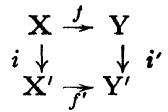
\includegraphics[keepaspectratio]{images/part002_3c8eaa6f.jpg}}

可交换，其中 \(i\) 与 \(i'\) 是典范映射。

对 \(i' \circ f: \mathbf{X} \to \mathbf{Y}'\) 应用命题 16。

一致空间的伴随 Hausdorff 空间也可以用下列性质来刻画：

命题 17 设 X 是一致空间，\(i(X)\) 是它的伴随 Hausdorff 空间，并设 \(f\) 是 X 到 Hausdorff 一致空间 \(X'\) 上的映射，使得 X 的一致结构是经由 \(f\) 从 \(X'\) 的一致结构取逆像而得的。则映射 \(g:i(X)\to X'\)（它使 \(f=g\circ i\)）是一个同构。

由命题 16，g 一致连续；g 显然是满射，并且也是单射，因为关系 \(f(x) = f(y)\) 按定义蕴含 \((x,y)\) 属于 X 的所有一致邻域，从而 \(i(x)=i(y)\)（第 7 目命题 12）。最后，\(X'\) 的一致邻域是 X 的一致邻域在 \(f\times f\) 下的像（§ 2 第 4 目的注），因而它们也是经由 \(g\times g\) 从 \(i(\mathbf{X})\) 的一致邻域得到的像（第 7 目命题 12）；由此即得结论。

注。设 R 是 X 上的等价关系 \(i(x) = i(x')\)。我们已看到（第 7 目命题 12），R 的图像 C 是 X 的所有一致邻域之交。显然，X 中的每个开集（因而每个闭集）关于 R 是饱和的；考虑到拓扑的逆像的定义，我们断言，商空间 X/R 到 \(i(X)\) 上的典范双射（由 \(i\) 所诱导）是一个同胚。因此，作为拓扑空间，X 的伴随 Hausdorff 空间可与 X/R 等同。典范映射 \(i: X \to i(X)\) 是开的和闭的，甚至是逆紧的（第一章 § 10 第 2 目的例）。

设 \(X'\) 是另一个一致空间，\(C'\) 是 \(X'\) 的所有一致邻域之交，\(R'\) 是以 \(C'\) 为图像的等价关系。设 \(f: X \to X'\) 是连续映射。由于在 \(f\) 之下，\(f(x)\) 的任一邻域的逆像是 \(x\) 的邻域，可知在 \(f\) 之下 \(C'(f(x))\) 的逆像包含 \(C(x)\)，因此 \(f\) 与 \(R\) 及 \(R'\) 相容，并诱导出一个连续映射 \(X/R \to X'/R'\)（第一章 § 3 第 4 目命题 6 的推论）。这推广了命题 16 的推论。

\subsection{子空间与积空间的完备化}

命题 18 设 X 是一个集合，\((\mathbf{Y}_{\lambda})_{\lambda \in \mathbf{L}}\) 是一族一致空间，且对每个 \(\lambda \in \mathbf{L}\)，设 \(f_{\lambda}\) 是 X 到 \(\mathbf{Y}_{\lambda}\) 中的映射。设 X 赋有最粗的一致结构 \(\mathcal{U}\)，它使所有 \(f_{\lambda}\) 都一致连续。则 X 的 Hausdorff 完备化 \(\hat{\mathbf{X}}\) 的一致结构是使所有映射 \(\hat{f}_{\lambda} \colon \hat{\mathbf{X}} \to \hat{\mathbf{Y}}_{\lambda} (\lambda \in \mathbf{L})\)（第 7 目命题 15）都一致连续的最粗的一致结构。此外，若 \(j_{\lambda}\) 是 \(\mathbf{Y}_{\lambda}\) 到 \(\hat{\mathbf{Y}}_{\lambda}\) 中的典范映射，且 \(g_{\lambda} = j_{\lambda} \circ f_{\lambda}\)，则 \(\hat{\mathbf{X}}\) 可与 \(\prod_{\lambda \in \mathbf{L}} \hat{\mathbf{Y}}_{\lambda}\) 中 X 在映射 \(x \to (g_{\lambda}(x))\) 下的像的闭包等同起来。

设 \(X'\)（相应地 \(Y_{\lambda}'\)）是 \(X\)（相应地 \(Y_{\lambda}\)）的伴随 Hausdorff 一致空间，并设 \(f_{\lambda}' \colon X' \to Y_{\lambda}'\) 是使图表

\[
\begin{array}{c} \mathbf {X} \xrightarrow {f _ {\lambda}} \mathbf {Y} _ {\lambda} \\ i \downarrow \\ \mathbf {X ^ {\prime}} \xrightarrow [ f _ {j} ^ {I} ]{} \mathbf {Y} _ {\lambda} ^ {\prime} \end{array}
\]

可交换的一致连续映射（i 为典范映射）。

初始一致结构的传递性（§ 2 第 3 目命题 5）一方面表明，\(\mathcal{U}\) 是使映射 \(j_{\lambda} \circ f_{\lambda}: \mathbf{X} \to \mathbf{Y}_{\lambda}'\) 都一致连续的最粗一致结构；另一方面表明，\(\mathcal{U}\) 也是经由 \(i\) 从 \(\mathcal{U}'\)（即集合 \(\mathbf{X}'\) 上使诸 \(f_{\lambda}'\) 一致连续的最粗一致结构）取逆像而得。现在 \(\mathcal{U}'\) 是 Hausdorff 的，因为若 \(x_{1}, x_{2}\) 是 \(\mathbf{X}\) 的两点，使得 \(j_{\lambda}(f_{\lambda}(x_{1})) = j_{\lambda}(f_{\lambda}(x_{2}))\) 对每个 \(\lambda \in L\) 成立，则 \((x_{1}, x_{2})\) 属于 \(\mathcal{U}\) 的所有一致邻域，从而 \(i(x_{1}) = i(x_{2})\)。于是第 8 目命题 17 表明，\(\mathcal{U}'\) 是伴随 Hausdorff 空间 \(\mathbf{X}'\)（\(\mathbf{X}\) 的）的一致结构。

在此情形下，双射 \(x' \to (f_{\lambda}'(x'))\) 把 X 等同于积 \(\prod_{\lambda} Y_{\lambda}'\) 的一个一致子空间（ \(\S\) 2 第 6 目命题 8）。由于诸 \(Y_{\lambda}'\) 是 Hausdorff 的，每个 \(Y_{\lambda}'\) 可与其完备化 \(\hat{Y}_{\lambda}\) 的一个稠密子空间等同，从而 \(\prod_{\lambda} Y_{\lambda}'\) 可与 \(\prod_{\lambda} \hat{Y}_{\lambda}\) 的一个稠密子空间等同（第一章 § 4 第 3 目命题 7）。但 \(\prod_{\lambda} \hat{Y}_{\lambda}\) 是 Hausdorff 的且完备的（第 5 目命题 10）；因此闭包 \(\overline{X}'\)（即 \(X'\) 在 \(\prod_{\lambda} \hat{Y}_{\lambda}\) 中的闭包）是完备 Hausdorff 子空间（第 4 目命题 8），它可与 X 的 Hausdorff 完备化 \(\hat{X}\) 等同；在这一等同之下，诸映射 \(\hat{f}_{\lambda}\) 成为到因子 \(\hat{Y}_{\lambda}\) 上的投影，命题得证。

推论 1 设 X 是一致空间，i 是 X 到其 Hausdorff 完备化 \(\hat{X}\) 中的典范映射；设 A 是 X 的子空间，j: A → X 是典范单射。则 j: \(\hat{A} \rightarrow \hat{X}\) 是 \(\hat{A}\) 到 i(A) 在 \(\hat{X}\) 中的闭包上的一个同构。

推论 2 设 \((\mathbf{Y}_{\lambda})_{\lambda \in \mathbf{L}}\) 是一族一致空间。则积空间 \(\prod_{\lambda \in \mathbf{L}}\mathbf{Y}_{\lambda}\) 的 Hausdorff 完备化典范地同构于积 \(\prod_{\lambda \in \mathbf{L}}\hat{\mathbf{Y}}_{\lambda}\)。

\section{一致空间与紧空间之间的关系}

\subsection{紧空间的一致结构}

定义 1 拓扑空间 X 上的一致结构称为与 X 的拓扑相容，如果后者与该一致结构诱导的拓扑重合。

若拓扑空间上存在与它的拓扑相容的一致结构，则称该拓扑空间为可一致化的，并称其拓扑为可一致化的。

存在不可一致化的拓扑空间，例如任何不满足公理 \((\mathrm{O}_{\mathrm{III}})\) 的空间（§ 1 第 2 目命题 2 的推论 3）；于是就产生了在什么条件下一个拓扑空间可一致化的问题。

我们要到第九章 § 1 才给出这个问题的完整回答。在本节中我们只考察一个重要的特殊情形，即 X 是紧空间的情形。这时我们有下面的定理：

定理 1 在紧空间 X 上，恰有一个与 X 的拓扑相容的一致结构；这个一致结构的一致邻域是对角线 \(\Delta\)（在 \(\mathbf{X} \times \mathbf{X}\) 中的）的所有邻域。此外，赋有这个一致结构的 X 是完备一致空间。

定理的最后一部分是直接的；因为 X 上的每个 Cauchy 滤子都有聚点{[}公理 (C){]}，因而收敛（§ 3 第 2 目命题 5 推论 2）。

我们接着证明，若 X 上存在与 X 的拓扑相容的一致结构，则它的一致邻域组成的集 U 是 \(\Delta\) 的所有邻域组成的集。我们已知每个一致邻域都是 \(\Delta\) 的邻域（§ 1 第 2 目命题 2），因此只需证明反之每个 \(\Delta\) 的邻域都属于 U。假设存在 \(\Delta\) 的一个不属于 U 的邻域 U；则当 V 取遍 U 时，诸集合 \(V \cap CU\) 构成紧空间 \(X \times X\) 上一个滤子 G 的基；于是 G 有一个聚点 \((a, b)\)（不属于 \(\Delta\)）。由于 U 是比 G 粗的滤子，\((a, b)\) 也是 U 的聚点。但按假设由 U 定义的一致结构是 Hausdorff 的；因此 U 的诸集合的闭包之交是 \(\Delta\)（§ 1 第 2 目命题 2 的推论 2 及命题 3）；于是我们得到矛盾。

因此剩下要证明的是，\(\mathfrak{B}\)（即 \(\Delta\) 在 \(\mathbf{X} \times \mathbf{X}\) 中的邻域组成的集）是某个与 \(\mathbf{X}\) 的拓扑相容的一致结构的一致邻域集。为此只需证明 \(\mathfrak{B}\) 是 \(\mathbf{X}\) 上某个 Hausdorff 一致结构的一致邻域集；因为这时该一致结构诱导的拓扑将比 \(\mathbf{X}\) 的拓扑粗（第一章 § 2 第 2 目命题 3），从而必与后者重合（第一章 § 9 第 4 目定理 2 推论 3）。

\(\mathfrak{B}\) 显然满足公理 \((\mathbf{F}_{\mathrm{I}})\) 与 \((\mathbf{F}_{\mathrm{II}})\)。我们来证明公理 \((\mathbf{U}_{\mathrm{II}})\) 与 \((\mathbf{U}_{\mathrm{III}})\) 也得到满足，并且 \(\Delta\) 是 \(\mathfrak{B}\) 中诸集合之交。先证最后一点：每个由单独一点 \((x, y) \in \mathbf{X} \times \mathbf{X}\) 组成的集合都是闭的，因为 \(\mathbf{X}\) 是 Hausdorff 的；因此若 \(x \neq y\)，则 \((x, y)\) 在 \(\mathbf{X} \times \mathbf{X}\) 中的余集是 \(\Delta\) 的邻域。由于对称映射 \((x, y) \to (y, x)\) 是 \(\mathbf{X} \times \mathbf{X}\) 到自身的同胚，可知 \(V \in B\) 蕴含 \(\overline{V} \in B\)，由此得 \((U_{II})\)。最后，假设 \((U_{III})\) 不满足；则存在集合 \(V \in B\)，使得对所有 \(W \in B\)，集合 \(\overline{W} \cap C V\) 非空；于是当 W 取遍 B 时，诸集合 \(\overline{W} \cap C V\) 构成 \(X \times X\) 上的一个滤子基，且该滤子基有一个聚点 \((x, y)\)（不在 \(\Delta\) 中）。现在，由于 X 是正则的（第一章 §9 第 2 目命题 1 的推论），存在不相交的开邻域 \(U_{1}\)（x 的）与 \(U_{2}\)（y 的），并且存在闭邻域 \(V_{1} \subset U_{1}\) 与 \(V_{2} \subset U_{2}\)（分别为 x 与 y 的闭邻域）。令 \(U_{3} = C(V_{1} \cup V_{2})\)，并考虑邻域

\[
\mathbf {W} = \bigcup_ {i = 1, 2, 3} (\mathrm{U} _ {i} \times \mathrm{U} _ {i}) \text {of} \Delta \text {in} \mathbf {X} \times \mathbf {X}.
\]

由这些定义立即得出，若 \((u, v) \in W\) 且 \(u \in V_1\)（相应地 \(u \in U_1\)），则必有 \(v \in U_1\)（相应地 \(v \in U_1 \cup U_3 = \complement V_2\)）；因此邻域 \(V_1 \times V_2\)（\((x, y)\) 在 \(X \times X\) 中的）不与 \(W\) 相交，这就得到矛盾。证明完毕。

注 1 对每个有限开覆盖 \(\Re = (\mathrm{U}_i)_{1\leqslant i\leqslant n}\)（\(\mathbf{X}\) 的），集合

\[
\mathrm{V} _ {\Re} = \bigcup_ {i = 1} ^ {n} \left(\mathrm{U} _ {i} \times \mathrm{U} _ {i}\right)
\]

是 \(\Delta\)（在 \(\mathbf{X} \times \mathbf{X}\) 中的）的邻域，并且这些集合 \(\mathrm{V}_{\Re}\) 构成 \(\Delta\) 的一个基本邻域系（因而构成 \(\mathbf{X}\) 上唯一一致结构的一致邻域基本系）。设 \(\mathbf{W}\) 是 \(\Delta\) 在 \(\mathbf{X} \times \mathbf{X}\) 中的任一邻域；则对每个 \(x \in \mathbf{X}\)，存在开邻域 \(\mathbf{U}_x\)（\(x\) 在 \(\mathbf{X}\) 中的），使 \(\mathbf{U}_x \times \mathbf{U}_x \subset \mathbf{W}\)。由于诸 \(\mathbf{U}_x\)（ \(x \in \mathbf{X}\) ）构成 \(\mathbf{X}\) 的开覆盖，故存在有限多个点 \(x_i\)（ \(1 \leqslant i \leqslant n\) ）使诸 \(\mathbf{U}_{x_i}\)（ \(1 \leqslant i \leqslant n\) ）构成一个覆盖 \(\Re\)（\(\mathbf{X}\) 的）。于是有 \(\mathrm{V}_{\Re} \subset \mathrm{W}\)，这就证明了所述断言。

由于这个原因，X 上唯一的一致结构常称为有限开覆盖的一致结构（参看第九章 § 4 习题 17）。

推论 1 紧空间的每个子空间都是可一致化的。

推论 2 每个局部紧空间都是可一致化的。

因为由 Alexandroff 定理（第一章 § 9 第 8 目定理 4），局部紧空间同胚于紧空间的子空间。

注 2 可能发生这样的情形：与局部紧空间的拓扑相容的一致结构不止一个且互不相同。

例如，我们已经看到，在无限离散空间上，有多于一个相容于离散拓扑的不同一致结构（§ 2 第 2 目的注）。

尽管如此，与可一致化空间的拓扑相容的一致结构的唯一性并不是刻画紧空间的性质；存在不紧但其一致结构唯一的局部紧空间（习题 4）。

定理 2 每个连续映射 \(f\)（从紧空间 \(X\) 到一致空间 \(X'\) 中的）都是一致连续的。

令 \(g = f \times f\)，则 \(g\) 在 \(X \times X\) 上连续（第一章 § 4 第 1 目命题 1 推论 1）；因此对每个开一致邻域 \(V'\)（\(X'\) 的），\(\overline{g}(V')\) 是 \(X \times X\) 的开子集，它显然包含对角线。于是定理由定理 1 得出，因为 \(X'\) 的开一致邻域构成一个一致邻域基本系（§ 1 第 2 目命题 2 推论 2）。

在定理 2 的假设下，\(f\) 在任一子空间 \(A\)（\(X\) 的）上的限制是一致连续的；因此（§ 3 第 6 目定理 2）：

推论 设 A 是紧空间 X 的稠密子空间，f 是 A 到完备 Hausdorff 一致空间 X' 中的映射。则 f 可由连续性延拓到整个 X 上，当且仅当 f 一致连续。

\subsection{一致空间的紧性}

定义 2 一致空间 X 称为准紧的，如果它的 Hausdorff 完备化 \(\hat{\mathbf{X}}\) 是紧的。一致空间 X 的子集 A 称为准紧子集，如果 X 的一致子空间 A 是准紧的。

于是，一致空间 X 的子集 A 是准紧的，当且仅当 \(i(\mathbf{A})\) 在 \(\hat{X}\) 中的闭包是紧的（ \(i: X \rightarrow \hat{X}\) 为典范映射）（ \(\S\) 3 第 9 目命题 18 推论 1）。

例。在任何一致空间 X 中，Cauchy 序列 \((x_{n})\) 的点组成的集是准紧的。由于诸 \(x_{n}\) 在 \(\hat{X}\) 中的像仍构成 Cauchy 序列，我们可以假定 X 是 Hausdorff 的；于是在 \(\hat{X}\) 中，由诸点 \(x_{n}\) 组成的集的闭包由诸点 \(x_{n}\) 与 \(\lim_{n\to\infty}x_{n}\) 组成，因而是紧的（第一章 § 9 第 3 目例 2）。

定理 3 一致空间 X 是准紧的，当且仅当对 X 的每个一致邻域 V，存在 X 的一个由 V-小集组成的有限覆盖。

我们可以更直观地把这个条件表述为：X 可以被有限多个集覆盖，而这些集要多么小就可以多么小。

设 \(i: \mathbf{X} \to \hat{\mathbf{X}}\) 为典范映射，则 \(\mathbf{X}\) 的一致邻域是经由 \(i \times i\) 从 \(\hat{\mathbf{X}}\) 的一致邻域取逆像而得的集合（§ 3 第 7 目命题 12）。设 \(\mathbf{X}\) 准紧，并设 \(\mathbf{U}\) 为任一一致邻域（\(\hat{\mathbf{X}}\) 的）；则存在一个对称一致邻域 \(\mathbf{U}'\)（\(\hat{\mathbf{X}}\) 的），使 \(\hat{\mathbf{U}}' \subset \mathbf{U}\)。由于 \(\hat{\mathbf{X}}\) 是紧的，存在有限多个点 \(x_j \in \hat{\mathbf{X}}\) 使诸 \(\mathbf{U}'(x_j)\)（它们是 U-小集）覆盖 \(\hat{\mathbf{X}}\)。若 \(\mathbf{V}\) 是 \(\mathbf{U}\) 经由 \(i \times i\) 的逆像，则诸集合 \(i^{-1}(\mathbf{U}'(x_j))\) 是 V-小集且覆盖 \(\mathbf{X}\)。反之，假设对每个一致邻域 \(\mathbf{V}\)（\(\mathbf{X}\) 的），存在 \(\mathbf{X}\) 的一个由 V-小集组成的有限覆盖。我们要证明每个超滤子 \(\mathfrak{F}\)（\(\hat{\mathbf{X}}\) 上的）都收敛；由于 \(\hat{\mathbf{X}}\) 是完备的，只需证明 \(\mathfrak{F}\) 是 Cauchy 滤子，即对每个闭一致邻域 \(\mathbf{U}\)（\(\hat{\mathbf{X}}\) 的），在 \(\mathfrak{F}\) 中有一个 U-小集（§ 1 第 2 目命题 2 推论 2）。设 \(\mathbf{V}\) 是 \(\mathbf{U}\) 在 \(i \times i\) 下的逆像，并设 \((\mathbf{B}_j)\) 是 \(\mathbf{X}\) 的一个由 V-小集组成的有限覆盖；则诸集合 \(C_j = i(B_j)\) 是 U-小集且覆盖 \(i(\mathbf{X})\)，于是

\[
\hat {\mathbf {X}} = \bigcup_ {j} \overline {{\mathbf {C}}} _ {j}.
\]

另一方面，由于 \(\mathbf{C}_j \times \mathbf{C}_j \subset \mathbf{U}\)，且 \(\mathbf{U}\) 在 \(\hat{\mathbf{X}} \times \hat{\mathbf{X}}\) 中是闭的，故 \(\overline{\mathbf{C}}_j \times \overline{\mathbf{C}}_j \subset \mathbf{U}\)，从而诸 \(\overline{\mathbf{C}}_j\) 也是 \(\mathbf{U}\)-小集。由于 \(\mathfrak{F}\) 是超滤子，诸 \(\overline{\mathbf{C}}_j\) 之一属于 \(\mathfrak{F}\)（第一章 § 6 第 4 目命题 5 的推论）。

证毕。

推论 一致空间 X 是紧的，当且仅当它是 Hausdorff 的、完备的，并且能被有限多个 V-小集覆盖，其中 V 是 X 的任一一致邻域。

这由定理 3 及第 1 目的定理 1 得出。

注 1 非 Hausdorff 的拟紧空间未必可一致化，因为它未必满足公理 (O \(_{III}\) )（参看第一章 § 9 第 2 目）；例如代数几何中出现的大多数非 Hausdorff 拟紧空间都不满足公理 (O \(_{III}\) )（参看习题 2）。

命题 1 在一致空间中，准紧集的每个子集、准紧集的每个有限并以及每个准紧集的闭包都是准紧的。

前两个断言是定理 3 的直接推论。设 X 是一致空间，A 是 X 的准紧子集，并设 \(i: \mathbf{X} \to \hat{\mathbf{X}}\) 为典范映射。\(i(\overline{\mathbf{A}})\) 包含在 \(i(\mathbf{A})\) 于 \(\hat{\mathbf{X}}\) 中的闭包内（第一章 § 2 第 1 目定理 1），因此 \(i(\overline{\mathbf{A}})\) 在 \(\hat{\mathbf{X}}\) 中的闭包包含在一个紧集中，从而是紧的。

\pandocbounded{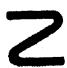
\includegraphics[keepaspectratio]{images/part002_3e3611b3.jpg}}

注 2 在一致空间 X 中，相对紧集 A 是准紧的，因为 A 包含在一个紧集中。另一方面，即使 X 是 Hausdorff 的，准紧集也未必在 X 中相对紧，X 本身准紧但不紧的情形就表明了这一点。

命题 2 设 \(f: \mathbf{X} \to \mathbf{Y}\) 是一致连续映射。若 \(\mathbf{A}\) 是 \(\mathbf{X}\) 的任一准紧子集，则 \(f(\mathbf{A})\) 是 \(\mathbf{Y}\) 的准紧子集。因为若 \(i: \mathbf{X} \to \hat{\mathbf{X}}\) 与 \(j: \mathbf{Y} \to \hat{\mathbf{Y}}\) 为典范映射，我们有 \(j(f(\mathbf{A})) = \hat{f}(i(\mathbf{A}))\)（§ 3 第 7 目命题 15），因而 \(j(f(\mathbf{A}))\) 在 \(\hat{\mathbf{Y}}\) 中相对紧（第一章 § 9 第 4 目定理 2 推论 1）。

命题 3 设 X 是一个集合，\((\mathrm{Y}_{\lambda})_{\lambda \in \mathbf{L}}\) 是一族一致空间，且对每个 \(\lambda \in L\)，设 \(f_{\lambda}\) 是 X 到 \(Y_{\lambda}\) 中的映射。设 X 赋有使诸 \(f_{\lambda}\) 一致连续的最粗一致结构。则 X 的子集 A 是准紧的，当且仅当 \(f_{\lambda}(A)\) 是 \(Y_{\lambda}\) 的准紧子集（对每个 \(\lambda \in L\)）。

这个条件由命题 2 知是必要的。充分性由 § 3 第 9 目命题 18 给出的 X 的 Hausdorff 完备化的刻画以及 Tychonoff 定理（第一章 § 9 定理 3 的推论）得出。

\subsection{一致空间中的紧集}

下面这个关于任意一致空间的命题，是第一章 § 9 第 2 目命题 2 对紧空间的更精确形式。

命题 4 在一致空间 X 中，设 A 是紧集，B 是闭集，且 A∩B=∅。则存在 X 的一致邻域 V，使 V(A) 与 V(B) 不相交。

若命题不真，则当 V 取遍 X 的对称一致邻域时，诸集合 \(A \cap \mathring{V}(B)\) 都不空；于是这些集合将在 A 上构成一个滤子基，它有一个聚点 \(x_0 \in A\)。因此对每个对称一致邻域 \(V\)（\(X\) 的），\(\dot{V}(x_0)\) 将与 \(B\) 相交，从而由于 \(B\) 是闭的，应有 \(x_0 \in B\)，与假设矛盾。

推论 设 A 是一致空间 X 中的紧集；则当 V 取遍 X 的一致邻域时，诸集合 V(A) 构成 A 的一个基本邻域系。

设 U 是 A 的任一开邻域，则 B = CU 是闭的且不与 A 相交；于是由命题 4，存在一致邻域 V 使 \(\mathrm{V}(\mathrm{A}) \cap \mathrm{V}(\mathrm{B}) = \varnothing\)，因此 \(\mathrm{V}(\mathrm{A}) \subset \mathrm{U}\)。

\subsection{紧空间中的连通集}

定义 3 设 V 是一致空间 X 的对称一致邻域。X 的点的有限序列 \((x_{i})_{0\leqslant i\leqslant n}\) 称为一条 V-链，如果 \(x_{i}\) 与 \(x_{i+1}\) 对 \(0\leqslant i<n\) 是 V-邻近的。点 \(x_{0}\) 与 \(x_{n}\) 称为该 V-链的端点，并称它们由这条 V-链连接。

给定对称一致邻域 V，关系“存在一条连接 x 与 y 的 V-链”是 X 中 x 与 y 之间的一个等价关系。设 \(A_{x,v}\) 是 x 关于这个关系的等价类，即可由一条 V-链与 x 连接的所有 \(y \in X\) 组成的集。显然，若 \(y \in A_{x,v}\)，则 \(\mathrm{V}(y) \subset \mathrm{A}_{x,\mathrm{v}}\)；因此 \(A_{x,v}\) 在 X 中是开的；而 \(A_{x,v}\) 的余集作为一些等价类的并，也是开的。于是：

命题 5 在一致空间 X 中，可与给定点 x 由 V-链连接的点组成的集 \(A_{x,v}\) 在 X 中既开又闭。

对每个 \(x \in X\)，设 \(A_{x}\) 表示当 V 取遍 X 的对称一致邻域时诸集合 \(A_{x,v}\) 的交；\(A_{x}\) 是 x 关于等价关系“对一切对称一致邻域 V，存在一条连接 x 与 y 的 V-链”的等价类。

命题 6 在紧空间 X 中，x 的连通分支、集合 \(A_{x}\)、以及 x 的既开又闭的邻域的交，这三者是同一个集合。

只需证明 \(A_{x}\) 是连通的：因为在任意一致空间 X 中，x 的连通分支包含在 x 的既开又闭的邻域的交中，而这个交由命题 5 包含在 \(A_{x}\) 中。

假设 \(A_{x}\) 不连通。由于 \(A_{x}\) 是闭的，存在两个不相交的非空闭集 B 与 C，使 \(B \cup C = A_{x}\)。由 §3 的命题 4，存在 X 的一致邻域 U 使 \(U(B) \cap U(C)\) 为空。

设 W 是开的一致邻域，使 \(\hat{W} \subset U\)，并设 H 是闭集，即 \(W(B) \cup W(C)\) 在 X 中的余集。例如设 \(x \in B\)，并设 y 是 C 的一点。则对每个对称一致邻域 \(V \subset W\)，由 W 的取法，对 i 用归纳法立即看出，在 X 中连接 x 与 y 的每条 V-链 \((x_{i})_{0 \leqslant i \leqslant n}\) 必有一点在 H 中。由于按假设对每个对称一致邻域 V，x 与 y 都可由一条 V-链连接，可见 \(H \cap A_{x,v}\) 当 \(V \subset W\) 时不空。另一方面，若 \(V' \subset V\)，则显然 \(A_{x,v'} \subset A_{x,v}\)；由此可得，当 V 取遍 X 的对称一致邻域时，诸集合 \(H \cap A_{x,v}\) 在紧空间 H 中构成一个由闭集组成的滤子基。因此所有这些集合有一公共点，从而 H 与 \(A_{x}\) 相交；但这与 H 的定义矛盾。

推论 设 X 是局部紧空间，K 是 X 的紧连通分支。则 K 的既开又闭的邻域构成 K 的一个基本邻域系。

设 V 是 K 在 X 中的相对紧开邻域（第一章 § 9 第 7 目命题 10），并设 F 是它的边界。设 U ⊂ V 是一个关于 V 既开又闭的集合。则 U 在 X 中是闭的，且若此外 U 不与 F 相交，则 U 在 X 中是开的（因为这时 U ⊂ V 且 U 在 V 中是开的）。因此只需证明存在 V 的一个子集，它包含 K、不与 F 相交且关于 V 既开又闭。

假设情形不是这样：则 F 与 \(\overline{V}\) 的那些包含 K 且在 \(\overline{V}\) 中既开又闭的子集的交，在 F 中构成一个由闭集组成的滤子基；F 是紧的，故这些集合有一公共点 \(y \in F\)。但这是荒谬的；由于 \(\overline{V}\) 是紧的，K 是 \(\overline{V}\) 的一个连通分支，且由命题 6，\(\overline{V}\) 中那些包含 K 且既开又闭的集合的交恰好是 K。推论至此得证。

命题 7 设 X 是紧空间，R 是 X 上的等价关系，其类是 X 的连通分支。则商空间 X/R 是紧的且全不连通。

由第一章 § II 第 5 目命题 9 我们知道 X/R 是全不连通的；因此要证明 X/R 是 Hausdorff 的（第一章 § 10 第 4 目命题 8）。设 A 与 B 是 X 的两个不同的连通分支。由命题 6，存在 X 的对称一致邻域 U，使 A 的任何点都不能由一条 U-链与 B 的任何点连接。X 中可由一条 U-链与一点 \(x \in A\)（相应地 \(y \in B\)）连接的点组成的集 V（相应地 W）在 X 中既开又闭（命题 5）且包含 A（相应地 B）；因此这两个集合分别是 A 与 B 的开邻域，关于 R 是饱和的，且不相交。证明完毕。

\BourbakiExercises

\BourbakiExerciseGroup

\begin{enumerate}
\def\labelenumi{\arabic{enumi})}
\tightlist
\item
  设 X 是无限集，F 是 X 上的一个超滤子，且 F 中诸集之交为空。对每个 \(A \in F\)，设 \(V_{A}\) 表示子集 \(\Delta \cup (A \times A)\)（\(X \times X\) 的）。证明：当 A 取遍 F 时，诸集合 \(V_{A}\) 构成 X 上某个一致结构 \(\mathcal{U}(\mathfrak{F})\) 的一致邻域基本系，且该一致结构诱导的拓扑是离散拓扑。
\end{enumerate}

*2) 在带有加法一致结构的实直线 R 上，证明当 V 取遍 R 的一致邻域滤子时，诸集合 V(Z) 并不构成有理整数集 Z 的基本邻域系。*（参看 § 4 第 3 目命题 4 的推论）。

*3) 设 V 是 R 上加法一致结构中由所有对 \((x, y)\)（满足 \(|x - y| \leqslant 1\) 或 \(xy \geqslant 1\) 的）组成的一致邻域。证明 V 在 \(R \times R\) 中是闭的，但若 A 表示由所有整数 \(n \geqslant 2\) 组成的 R 的（闭）子集，则 \(V(A)\) 在 \(R\) 中不是闭的。*

\begin{enumerate}
\def\labelenumi{\arabic{enumi})}
\setcounter{enumi}{3}
\tightlist
\item
  证明若一致空间是 Kolmogoroff 空间（第一章 § 1 习题 2），则它是 Hausdorff 的。
\end{enumerate}

¶ 5) a) 设 X 是一致空间，U 是它的一致结构；对 X 的每个一致邻域 V，设 \(\tilde{V}\) 是 \(\mathfrak{P}(X) \times \mathfrak{P}(X)\) 的子集，由 X 的子集的所有满足 \(M \subset V(N)\) 且 \(N \subset V(M)\) 的对 (M, N) 组成。证明诸集合 \(\tilde{V}\) 构成某个一致结构 \(\tilde{U}\)（\(\mathfrak{P}(X)\) 上的）的一致邻域基本系。

\begin{enumerate}
\def\labelenumi{\alph{enumi})}
\setcounter{enumi}{1}
\item
  在集 \(\mathfrak{P}_{0}(\mathbf{X})\)（由 \(\mathbf{X}\) 的非空子集组成）上，证明由拓扑 \(\mathfrak{C}(\tilde{\mathcal{U}})\)（它由 \(\tilde{\mathcal{U}}\) 诱导）所诱导的拓扑比拓扑 \(\mathfrak{C}_{\Phi}\) 细（第一章 § 2 习题 7）。
\item
  若 X 至少有两点且 U 是 Hausdorff 的，证明 \(\mathfrak{G}(\tilde{\mathcal{U}})\) 在 \(\mathfrak{P}_{0}(\mathbf{X})\) 上诱导的拓扑决不比 \(G_{\Omega}\) 粗。\(\mathfrak{G}(\tilde{\mathcal{U}})\) 在由 X 的非空闭子集组成的集 \(\mathfrak{F}(\mathbf{X})\) 上诱导的拓扑比 \(G_{\Omega}\) 在这个集上诱导的拓扑细，当且仅当对 X 的每个闭子集 A，当 V 取遍 X 的一致邻域时诸集合 V(A) 构成 A 的一个基本邻域系。
\end{enumerate}

*d) 证明在第一章 § 11 习题 18 定义的商集 X/R 上，商拓扑以及由 \(\mathfrak{C}_{\Omega}\)、\(\mathfrak{C}_{\Phi}\) 与 \(\mathfrak{C}(\tilde{\mathcal{U}})\)（其中 \(\mathcal{U}\) 是 \(\mathbf{R}^2\) 上的通常一致结构）定义的拓扑，这四个拓扑互不相同。*

\BourbakiExerciseGroup

\(^{*}\) 1) 证明在实直线 R（带加法一致结构）上，函数 \(|x|\) 是一致连续的；函数 \(1/x\) 在每个区间 \([a, +\infty[\)（其中 a \textgreater{} 0）上一致连续；而这个函数在区间 \(]0, +\infty[\cdot*\)

\begin{enumerate}
\def\labelenumi{\arabic{enumi})}
\setcounter{enumi}{1}
\item
  证明由 p 进一致结构在 Z 上诱导的拓扑对不同的素数 p 是不可比较的。
\item
  设 \(\mathfrak{F}_1, \mathfrak{F}_2\) 是无限集 X 上两个不同的超滤子。证明一致结构 \(\mathcal{U}(\mathfrak{F}_1)\) 与 \(\mathcal{U}(\mathfrak{F}_2)\)（ \(\S\) I 习题 I）不可比较，且它们的上确界是离散一致结构。它们的下确界是什么？由此推出 X 上 Hausdorff 一致结构的全体与 \(\mathfrak{P}(\mathfrak{P}(X))\) 等势{[}参看第一章 \(\S\) 8 习题 6 a){]}。
\item
  \begin{enumerate}
  \def\labelenumii{\alph{enumii})}
  \tightlist
  \item
    设 \(\mathfrak{U}\) 与 \(\mathfrak{U}'\) 是同一个非空集 \(\mathbf{X}\) 上两个一致结构的一致邻域滤子。证明滤子 \(\mathfrak{U}\) 与 \(\mathfrak{U}'\) 的交是 \(\mathbf{X}\) 上某个一致结构的一致邻域滤子，当且仅当对每个 \(\mathbf{V} \in \mathfrak{U}\) 与 \(\mathbf{V}' \in \mathfrak{U}'\)，存在 \(\mathbf{W} \in \mathfrak{U}\) 与 \(\mathbf{W}' \in \mathfrak{U}'\) 使 \(\mathbf{WW}' \subset \mathbf{V} \cup \mathbf{V}'\)。
  \end{enumerate}
\end{enumerate}

\begin{enumerate}
\def\labelenumi{\alph{enumi})}
\setcounter{enumi}{1}
\tightlist
\item
  给出两个一致邻域滤子 \(\mathcal{U}_{\overline{\omega}}\)、\(\mathcal{U}_{\overline{\omega}'}\) 的例子，它们各由 X 的一个有限分拆定义（第 5 目的例），且不满足 \(a\) ) 中的条件。
\end{enumerate}

\begin{enumerate}
\def\labelenumi{\arabic{enumi})}
\setcounter{enumi}{4}
\tightlist
\item
  设 \((\mathbf{X}_i)_{i\in I}\) 是一族一致空间，\(c\) 是一个无限基数。对每个族 \((\mathbf{V}_i)_{i\in H}\)（其中 card \((\mathbf{H}) < c\)，且 \(\mathbf{V}_i\) 是 \(\mathbf{X}_i\) 的一致邻域（对每个 \(i\in H\)）），设 \(\mathbf{U}((\mathbf{V}_i))\) 为对 \((x,y)\)（\(\mathbf{X} = \prod_{i \in I}\mathbf{X}_i\) 的点的对）组成的集，满足 \((\mathrm{pr}_i x, \mathrm{pr}_i y) \in \mathbf{V}_i\) 对每个 \(i\in H\) 成立。
\end{enumerate}

证明诸集合 \(\mathbf{U}((\mathbf{V}_{i}))\) 构成 X 上某个一致结构的一致邻域基本系，且该一致结构诱导的拓扑就是第一章 § 4 习题 9 中定义的拓扑。

\begin{enumerate}
\def\labelenumi{\arabic{enumi})}
\setcounter{enumi}{5}
\tightlist
\item
  设 X 是一致空间，U 是它的一致结构，\(\tilde{U}\) 是 \(\mathfrak{P}(X)\) 上相应的一致结构（§ 1 习题 5）。
\end{enumerate}

\begin{enumerate}
\def\labelenumi{\alph{enumi})}
\item
  证明映射 \(x \to \{x\}\) 是一致空间 \(X\) 到一致空间 \(\mathfrak{P}(X)\) 的一个子空间上的同构。
\item
  证明 \(\widetilde{\mathcal{U}}\) 在集 \(\mathfrak{F}(\mathbf{X})\)（由 \(\mathbf{X}\) 的非空闭子集组成）上诱导的一致结构是 Hausdorff 的，并且 \(\widetilde{\mathcal{U}}\) 是经由映射 \(\mathbf{M} \to \overline{\mathbf{M}}\) 从 \(\widetilde{\mathcal{U}}\) 在 \(\mathfrak{F}(\mathbf{X})\) 上诱导的一致结构取逆像而得。c) 证明映射 \((\mathbf{M}, \mathbf{N}) \to \mathbf{M} \cup \mathbf{N}\)（从 \(\mathfrak{P}(\mathbf{X}) \times \mathfrak{P}(\mathbf{X})\) 到 \(\mathfrak{P}(\mathbf{X})\) 中）是一致连续的。
\item
  设 Y 是另一个一致空间。若 \(f: X \to Y\) 是一致连续映射，证明映射 \(M \to f(M)\)（从 \(\mathfrak{P}(X)\) 到 \(\mathfrak{P}(Y)\) 中）是一致连续的。
\item
  设 \(\mathfrak{M}\) 是集 \(\mathfrak{F}(\mathbf{X})\)（由 \(\mathbf{X}\) 的非空闭子集组成）的紧子集，\(\mathfrak{F}(\mathbf{X})\) 赋有由拓扑 \(\mathfrak{C}(\tilde{\mathcal{U}})\)（它由 \(\tilde{\mathcal{U}}\) 诱导）诱导的拓扑。证明集合 \(\bigcup_{\mathbf{M} \in \mathfrak{M}} \mathbf{M}\) 在 \(\mathbf{X}\) 中是闭的。
\end{enumerate}

\BourbakiExerciseGroup

\(^{*1}\) 设 U 表示实直线 R 上的加法一致结构，\(U'\) 表示 U 在 R 到自身的映射 \(x \rightarrow x^{3}\) 下的逆像。证明 \(U'\) 比 U 严格细，但两个一致结构的 Cauchy 滤子相同。\(^{*}\)

\begin{enumerate}
\def\labelenumi{\arabic{enumi})}
\setcounter{enumi}{1}
\tightlist
\item
  \begin{enumerate}
  \def\labelenumii{\alph{enumii})}
  \tightlist
  \item
    设 X 是无限集，F 是 X 上的非平凡超滤子。证明若 X 赋有一致结构 \(\mathcal{U}(\mathfrak{F})\)（§ 1 习题 1），则 X 在其完备化 \(\hat{X}\) 中的余集由单独一点组成，且拓扑空间 \(\hat{X}\) 可与超滤子 F 相伴的空间等同于（第一章 § 6 第 5 目的例）。
  \end{enumerate}
\end{enumerate}

*b) 由 a) 推出 R 上一个一致结构的例子，它比加法一致结构细，且 R 关于它不完备。*

*3) a) 设 \(\mathcal{U}\) 表示实直线 \(\mathbf{R}\) 上的加法一致结构，\(\mathcal{U}_1\) 表示 \(\mathbf{R}\) 上由扩充实直线 \(\overline{\mathbf{R}}\) 的一致结构诱导的一致结构，\(\mathcal{U}_2\) 表示 \(\mathbf{R}\) 上由单点紧化 \(\tilde{\mathbf{R}} = \mathbf{P}_1(\mathbf{R})\)（\(\mathbf{R}\) 的）的一致结构诱导的一致结构。证明 \(\mathcal{U}\) 比 \(\mathcal{U}_1\) 严格细，\(\mathcal{U}_1\) 比 \(\mathcal{U}_2\) 严格细，且这三个一致结构诱导的拓扑相同；又 \(\mathbf{R}\) 关于这三个一致结构的完备化分别是 \(\mathbf{R}\)、\(\overline{\mathbf{R}}\) 与 \(\tilde{R}\)。R 的恒等映射由连续性延拓为一个单而非满的映射 \(R \rightarrow \overline{R}\) 以及一个满而非单的映射 \(\overline{R} \rightarrow \tilde{R}\)。

\begin{enumerate}
\def\labelenumi{\alph{enumi})}
\setcounter{enumi}{1}
\tightlist
\item
  由 a) 推出一个例子：两个 Hausdorff 一致空间 X、Y 以及一个一致连续双射 \(u: X \rightarrow Y\)，其连续延拓 \(\overline{u}: \hat{X} \rightarrow \hat{Y}\) 既非单又非满。*
\end{enumerate}

¶ 4) 用 § 2 习题 5 的记号，假设所有一致空间 \(X_i\) 都完备。证明空间 \(X\) 关于那里定义的一致结构是完备的（用反证法，利用 § 2 命题 5 推论 2）。

\begin{enumerate}
\def\labelenumi{\arabic{enumi})}
\setcounter{enumi}{4}
\item
  设 X 是 Hausdorff 一致空间，且 X 是 \(\hat{X}\) 的可数个开集之交。证明若 Y 是任一以 X 为一致子空间的 Hausdorff 一致空间，则 X 是 Y 的一个闭子集与 Y 的可数个开集之交。
\item
  设 X 是一致空间，\(i: X \to \hat{X}\) 是 X 到其 Hausdorff 完备化中的典范映射。设 \(X_{0}\) 是 X 与 \(\hat{X} - i(X)\) 的和，\(j: X_{0} \to \hat{X}\) 是在 X 上与 i 一致、在 \(\hat{X} - i(X)\) 上与恒等映射一致的映射。证明 \(X_{0}\) 关于经由 j 从 \(\hat{X}\) 的一致结构取逆像而得的一致结构是完备的；又若 Y 是任一以 X 为一致子空间的完备一致空间，则恒等映射 \(X \to X\) 可唯一延拓为连续映射 \(X_{0} \to Y\)。
\end{enumerate}

¶ 7) 设 \(\mathbf{X}\) 是 Hausdorff 一致空间，\(\mathcal{U}\) 是它的一致结构，\(\mathcal{U}_0\) 是 \(\mathfrak{F}(\mathbf{X})\) 上由一致结构 \(\tilde{\mathcal{U}}\) 诱导的一致结构（ \(\S\) 2 习题 6 b)），\(\mathcal{U}_{00}\) 是 \(\mathfrak{F}(\mathfrak{F}(\mathbf{X}))\) 上由一致结构 \(\tilde{\mathcal{U}}_0\) 诱导的一致结构。证明典范映射 \(x \to \{\{x\}\}\)（从 \(\mathbf{X}\) 到 \(\mathfrak{F}(\mathfrak{F}(\mathbf{X}))\) 中的）可延拓为 \(\hat{\mathbf{X}}\) 到 \(\mathfrak{F}(\mathfrak{F}(\mathbf{X}))\) 的一个闭一致子空间（赋有一致结构 \(\mathcal{U}_{00}\)）上的同构（利用第 4 目命题 9）。

\BourbakiExerciseGroup

¶ 1) 设 R 是紧空间 X 的开覆盖。证明存在 X 的一致结构的一致邻域 V，使对每个 \(x \in X\)，\(V(x)\) 包含在属于 R 的某个集中{[}注意：对每个 \(x \in X\) 存在一致邻域 \(W_x\) 使 \(\dot{W}_x(x)\) 包含在 R 的某个集中，并用有限多个集 \(W_x(x)\) 覆盖 X{]}。

\begin{enumerate}
\def\labelenumi{\arabic{enumi})}
\setcounter{enumi}{1}
\item
  证明拟紧空间 X 可一致化，当且仅当它的拓扑是紧空间 Y 的拓扑在一个满射 \(f: X \rightarrow Y\) 下的逆像。
\item
  设 \(f\) 是紧空间 \(\mathbf{X}\) 到紧空间 \(\mathbf{Y}\) 中的连续映射，\(\mathbf{V}\) 是 \(\mathbf{X}\) 的开一致邻域，使得关系 \(f(x) = f(y)\) 蕴含 \((x, y) \in \mathbf{V}\)。证明存在一致邻域 \(W\)（\(\mathbf{Y}\) 的），使关系 \((f(x), f(y)) \in W\) 蕴含 \((x, y) \in V\)。
\item
  设 X 是第一章 § 9 习题 II 中定义的局部紧空间。证明对角线 \(\Delta\) 在 \(X \times X\) 中的每个邻域都包含一个形如 \([x, b[ \times [x, b[\) 的集。由此推出 X 上只有唯一一个与 X 的拓扑相容的一致结构，且 X 关于这个一致结构的完备化可与区间 \(X' = [a, b]\)（赋有拓扑 \(\mathcal{C}v(X)\)）等同。（注意 X 上的每个超滤子关于任何与 X 的拓扑相容的一致结构都必是 Cauchy 滤子）。
\item
  证明一致空间 X 是准紧的，当且仅当 X 上的每个超滤子都是 Cauchy 滤子。（注意：若 X 不准紧，则存在 X 的一致邻域 V，使当 x 取遍 X 时诸集合 \(\mathbb{C}\mathrm{V}(x)\) 在 X 上生成一个滤子）。
\item
  设 X 是这样一个一致空间：其中每个点列都至少有一个聚点。证明 X 是准紧的（用反证法）。
\item
  子集 \(\mathbf{A}\)（一致空间 \(\mathbf{X}\) 的）称为有界的，如果对每个一致邻域 \(\mathbf{V}\)（\(\mathbf{X}\) 的），存在有限集 \(\mathbf{F}\) 和整数 \(n > 0\) 使 \(\mathbf{A} \subset \overset{n}{\mathbf{V}}(\mathbf{F})\)。
\end{enumerate}

\begin{enumerate}
\def\labelenumi{\alph{enumi})}
\item
  两个有界子集的并是有界的。有界子集的闭包是有界的。每个准紧子集都是有界的。
\item
  若 \(f: \mathbf{X} \to \mathbf{Y}\) 一致连续，则在 \(f\) 下，\(\mathbf{X}\) 的每个有界子集的像是 \(\mathbf{Y}\) 的有界子集。
\item
  在非空一致空间的积中，一个集是有界的当且仅当它的每个投影都是有界的。
\item
  对 X 的每个对称一致邻域 V，设 \(R_{V}\) 表示诸集合 \(\stackrel{n}{V}\)（当 n 取遍整数 \textgreater0）的并。证明 \(R_{V}\) 在 \(X \times X\) 中既开又闭，且用第 4 目的记号，
\end{enumerate}

\[
\mathbf {R} _ {\mathbf {v}} (x) = \mathbf {A} _ {x, \mathbf {v}}
\]

对每个 \(x \in \mathbf{X}\) 成立。假设 \(\mathbf{R}_{\mathbf{V}} = \mathbf{X} \times \mathbf{X}\) 对每个对称一致邻域 \(\mathbf{V}\)（\(\mathbf{X}\) 的）都成立（特别当 \(\mathbf{X}\) 连通时就是这种情形）；证明集 \(\mathbf{A} \subset \mathbf{X}\) 有界当且仅当对每个对称一致邻域 \(\mathbf{V}\)（\(\mathbf{X}\) 的）与每个 \(x_0 \in \mathbf{X}\)，存在整数 \(n > 0\) 使 \(\mathbf{A} \subset \mathbf{V}(x_0)\)。

\begin{enumerate}
\def\labelenumi{\arabic{enumi})}
\setcounter{enumi}{7}
\item
  设 X 是一致空间，V 是 X 的闭一致邻域，A 是 X 的紧子集。证明 V(A) 在 X 中是闭的（参看第一章 § 10 第 2 目定理 1 推论 5）。
\item
  设 X 是局部紧空间，它带有一个与其拓扑相容的一致结构，并且存在一致邻域 V 具有如下性质：\(V(x)\) 对所有 \(x \in X\) 都在 X 中相对紧。a) 证明 X 关于这个一致结构是完备的。
\end{enumerate}

\begin{enumerate}
\def\labelenumi{\alph{enumi})}
\setcounter{enumi}{1}
\item
  设 \(\mathbf{U}\) 是 \(\mathbf{X}\) 的对称一致邻域，使 \(\dot{\mathbf{U}}\subset\mathbf{V}\)。证明若 \(\mathbf{A}\) 在 \(\mathbf{X}\) 中相对紧，则 \(\mathbf{U}(\mathbf{A})\) 亦然。
\item
  证明 X 是仿紧的{[}利用 b)、习题 7 及第一章 § 9 第 10 目定理 5{]}。
\item
  设 W 是 X 的闭对称一致邻域，使 \(\dot{W} \subset V\)。证明若 A 在 X 中闭，则 \(\mathbf{W}(\mathbf{A})\) 亦然（利用习题 8）。
\end{enumerate}

\begin{enumerate}
\def\labelenumi{\arabic{enumi})}
\setcounter{enumi}{9}
\tightlist
\item
  设 X 是 Hausdorff 一致空间，它有一个一致邻域 V，使 \(\mathbf{V}(x)\) 对每个 \(x \in X\) 都是准紧的。证明完备化 \(\hat{X}\) 是局部紧的且满足习题 9 的条件。{[}若 W 是 X 的对称开一致邻域，使 \(\hat{W} \subset V\)，证明闭包 \(\overline{W}\)（W 在 \(\hat{X} \times \hat{X}\) 中的）满足：\(\overline{W}(x)\) 对每个 \(x \in \hat{X}\) 是紧的{]}。
\end{enumerate}

¶ 11) 设 X 是 Hausdorff 一致空间，U 是它的一致结构，F(X) 是 X 的所有非空闭子集组成的集。设 F(X) 赋有由 § 1 习题 5 a) 中定义的一致结构 U 诱导的一致结构。

\begin{enumerate}
\def\labelenumi{\alph{enumi})}
\item
  证明若 \(X'\) 准紧，则 \(\mathfrak{F}(\mathbf{X})\) 亦然。{[}若 \((\mathbf{A}_{i})\) 是 X 的由 V-小集（V 对称）组成的有限覆盖，证明诸集合 \(\tilde{\mathbf{V}}(\mathbf{B}_{k})\) 覆盖 \(\mathfrak{F}(\mathbf{X})\)，其中诸 \(B_{k}\) 取遍诸集 \(A_{i}]\) 的所有并。
\item
  点 \(\mathbf{A} \in \mathfrak{F}(\mathbf{X})\) 具有如下性质：\(\mathbf{A}\) 在 \(\mathfrak{G}(\tilde{\mathcal{U}})\) 于 \(\mathfrak{F}(\mathbf{X})\) 上诱导的拓扑中的每个邻域，都包含 \(\mathbf{A}\) 在 \(\mathfrak{G}_{\Theta}\)（第一章 § 8 习题 12）于 \(\mathfrak{F}(\mathbf{X})\) 上诱导的拓扑中的一个邻域，当且仅当 \(\mathbf{A}\) 准紧。
\item
  证明拓扑 \(\mathfrak{G}(\mathfrak{U})\) 与 \(\mathfrak{G}_{\Theta}\) 在集 \(\mathfrak{K}(\mathbf{X})\)（由 \(\mathbf{X}\) 的紧子集组成）上诱导相同的拓扑{[}利用 \(b\) ) 及 §1 习题 5{]}。
\end{enumerate}

\begin{enumerate}
\def\labelenumi{\arabic{enumi})}
\setcounter{enumi}{11}
\tightlist
\item
  \begin{enumerate}
  \def\labelenumii{\alph{enumii})}
  \tightlist
  \item
    设 R 是一个布尔代数，并把 R 与 R 的极大预滤子组成的集 \(\Omega\) 的子集所成的布尔代数等同于（第一章 § 6 习题 20）。对每个有限分拆 \(\overline{\omega} = (\mathbf{A}_i)\)（\(\Omega\) 的，由属于 R 的集组成），设 \(\mathbf{C}_{\overline{\omega}}\) 表示子集 \(\bigcup_{i} (\mathbf{A}_i \times \mathbf{A}_i)\)（\(\Omega \times \Omega\) 的）。
  \end{enumerate}
\end{enumerate}

证明诸集合 \(C_{\overline{\omega}}\) 构成 \(\Omega\) 上某个 Hausdorff 一致结构的一致邻域基本系。完备化 \(\hat{\Omega}\)（\(\Omega\) 关于这个一致结构的）是一个全不连通紧空间。\(\hat{\Omega}\) 的子集在 \(\hat{\Omega}\) 中既开又闭，当且仅当它形如 \(\overline{\mathbf{A}}\)，其中 \(\mathbf{A} \in \mathbf{R}\)。证明 \(\mathbf{A} \to \overline{\mathbf{A}}\) 是 \(\mathbf{R}\) 到 \(\hat{\Omega}\) 的既开又闭子集全体上的双射，并且 \(\overline{\mathbf{C}}\mathbf{A} = \overline{\mathbf{C}}\overline{\mathbf{A}}\)，\(\overline{\mathbf{A} \cup \mathbf{B}} = \overline{\mathbf{A}} \cup \overline{\mathbf{B}}\) 与 \(\overline{\mathbf{A} \cap \mathbf{B}} = \overline{\mathbf{A}} \cap \overline{\mathbf{B}}\)。由此推出典范映射 \(\Omega \to \hat{\Omega}\) 是双射。

\begin{enumerate}
\def\labelenumi{\alph{enumi})}
\setcounter{enumi}{1}
\tightlist
\item
  设 X 是一个 Hausdorff 拓扑空间，其中既开又闭的集构成拓扑的基。取 R 为由 X 的既开又闭子集组成的布尔代数；则 \(\hat{\mathbf{X}}\)（X 关于一致结构 \(\mathcal{U}\)（在 \(a\) ) 中定义的）的完备化）的拓扑在 X 上诱导的拓扑就是 X 上给定的拓扑。此外，X 上以开集组成的集为基的滤子全体的极大元素，以及 X 上以闭集组成的集为基的滤子全体的极大元素，都是关于一致结构 \(\mathcal{U}\) 的 Cauchy 滤子。由此推出存在连续满射 \(\varphi: \hat{\mathbf{X}} \to \hat{\mathbf{X}}, \psi: \mathbf{X}' \to \hat{\mathbf{X}}\)，其中 \(\hat{\mathbf{X}}, \mathbf{X}'\) 是第一章 § 9 习题 25 与 24 中定义的空间。*证明若 X 是有理直线 Q，则 \(\psi\) 不是双射。*若 X 是极不连通的（第一章 § 11 习题 21），则 \(\psi\) 是双射，\(\hat{\mathbf{X}}\) 是极不连通的，并且可与伴随 \(\mathbf{X}'\) 的半正则空间等同于（第一章 § 8 习题 20）；于是极不连通空间可以刻画为极不连通紧空间的稠密子空间。试由此给出一个没有孤立点的极不连通紧空间的例子{[}（参看第一章 § 11 习题 21 f){]}。
\end{enumerate}

特别地，若取 X 为离散空间，则 \(\hat{X}\) 可与 X 的超滤子空间等同于（第一章 § 9 习题 26）。

13) 设 X 是局部紧空间，U 是 X 的开子集。设 B 是 U 与 CU 的相对紧连通分支的并。证明 B 是开的，且是 U 与 CU 的那些在 CU 中既开又紧的子集的并。（把 X 嵌入它的单点紧化 \(X' = X \cup \{\omega\}\)，注意在 \(X' - U\) 中 \(\omega\) 的连通分支是 \(\{\omega\} \cup CB\)，并利用第 4 目命题 6）。

\begin{enumerate}
\def\labelenumi{\arabic{enumi})}
\setcounter{enumi}{13}
\item
  设 X 是紧空间，B 是 X 上由连通闭集组成的滤子基。证明 B 中诸集之（非空）交是闭且连通的（用反证法，利用第 3 目命题 4 及第一章 § 9 第 1 目定理 1）。
\item
  设 X 是紧空间。则 X 的非空闭子集组成的空间 \(\mathfrak{F}(\mathbf{X})\)，赋有由 \(\mathcal{C}(\tilde{\mathcal{U}})\) 诱导的拓扑（习题 11），是紧的（第一章 § 9 习题 13）。考察一个超滤子 \(\Psi\)（\(\mathfrak{F}(\mathbf{X})\) 上的），并假设对 X 的一致结构的每个一致邻域 V 与每个 \(\mathfrak{X} \in \Psi\)，存在 \(\mathbf{M} \in \mathfrak{X}\) 使 \(\mathbf{M}\) 的任何两点都可由一条包含在 \(\mathbf{M}\) 中的 V-链连接。证明 \(\Psi\) 在 \(\mathfrak{F}(\mathbf{X})\) 中的极限点 A 是 \(\mathbf{X}\) 的连通子集（利用第 4 目命题 6）。
\item
  设 X 是连通紧空间，A、B 是 X 的两个不相交的非空闭子集。证明存在 \(\mathbb{C}(\mathrm{A} \cup \mathrm{B})\) 的一个连通分支，其闭包与 A 和 B 都相交。（设 U 是 X 的一致结构的一致邻域，使 \(\overline{\mathbf{U}}(\mathbf{A}) \cap \overline{\mathbf{U}}(\mathbf{B}) = \varnothing\)。首先证明集 \(\mathfrak{M}_{\mathrm{U}}\)（即 \(\overline{\mathbb{C}(\mathrm{U}(\mathbf{A}) \cup \mathrm{U}(\mathbf{B}))}\) 的既与 \(\overline{\mathrm{U}(\mathbf{A})}\) 相交又与 \(\overline{\mathrm{U}(\overline{\mathrm{B}})}\) 相交的连通分支组成的集）非空，办法是证明：对每个对称一致邻域 W ⊂ U，存在 \(x \in \mathrm{U}(\mathbf{A})\) 与 \(y \in \mathrm{U}(\mathbf{B})\) 以及一条连接 x 与 y 的 W-链，其除 x 与 y 外的所有点都属于 \(\mathbb{C}(\mathrm{U}(\mathbf{A}) \cup \mathrm{U}(\mathbf{B}))\)，然后应用习题 15。对每个一致邻域 V ⊂ U，证明每个 K ∈ \(\mathfrak{M}_{\mathrm{V}}\) 包含一个集 H ∈ \(\mathfrak{M}_{\mathrm{U}}\)，并且集 \(\mathfrak{M}_{\mathrm{U},\mathrm{V}}\)（由诸集 H ∈ \(\mathfrak{M}_{\mathrm{U}}\)（包含在某个集 K ∈ \(\mathfrak{M}_{\mathrm{V}}\) 中的）组成）在 \(\mathfrak{F}(\overline{\mathrm{X}})\) 中是闭的；最后推出，当 V 取遍包含在 U 中的一致邻域时，诸集 \(\mathfrak{M}_{\mathrm{U},\mathrm{V}}\) 的交非空）。
\item
  设 X 是连通局部紧空间。设 K 是 X 的任一非空紧子集且 K ≠ X。证明 K 的每个连通分支都与 K 在 X 中的边界相交（利用第 4 目命题 6 的推论）。由此推出，若 A 是 X 的任一非空相对紧开子集且 A ≠ X，则 A 的每个连通分支的闭包与 CA 相交。
\end{enumerate}

¶ 18) a) 证明紧连通空间 X 不能是可数无穷多个互不相交的非空闭集的并{[}用反证法：若 (F \(_{n}\) ) 是 X 的一个由闭集组成的可数无穷分拆，借助习题 17 证明存在紧连通集 K，它不与 F \(_{1}\) 相交但与无穷多个集 F \(_{n}\) 相交；为此考察 F \(_{2}\) 的一点关于 F \(_{2}\) 的一个紧邻域（不与 F \(_{1}\) 相交的）的连通分支。然后使用归纳法{]}。

\begin{enumerate}
\def\labelenumi{\alph{enumi})}
\setcounter{enumi}{1}
\tightlist
\item
  在下列两个附加条件之一成立时，把 a) 的结果推广到局部紧连通空间 X：某个 \(F_{n}\) 是紧且连通的，或者 X 是局部连通的。{[}在第一种情形，借助习题 17 化归为 a){]}。
\end{enumerate}

\(^{*}c)\) 设 \(\mathbf{X}\) 是 \(\mathbb{R}^3\) 的子空间，它是下列子空间的并：\(A_n\) 是半直线 \(x > 0\)，\(y = 1/n\)，\(z = 0\)（ \(n \geqslant 1\)）；\(B_n\) 是区间 \(2n < x < 2n + 2\)，\(y = 0\)，\(z = 0\)（ \(n \geqslant 0\)）；\(C_n\) 是由关系式

\[
x = 2 n + 1, \quad 0 \leqslant y \leqslant \frac {1}{n + 1}, \quad z = y \left(y - \frac {1}{n + 1}\right),
\]

所定义的集，其中 \(n \geqslant 0\)。

证明 X 是连通且局部紧的，并且是可数无穷多个互不相交的连通非空闭集的并。*

¶ 19) 紧连通空间 X 称为在它的两点 x, y 之间不可约的，如果除 X 自身外，X 的紧连通子集中没有同时包含 x 与 y 的。

\begin{enumerate}
\def\labelenumi{\alph{enumi})}
\item
  若 \(x\) 与 \(y\) 是紧连通空间 \(X\) 的两个不同点，证明 \(X\) 有一个紧连通子空间 \(K\)（在 \(x\) 与 \(y\) 之间不可约的）（利用习题 14 与 Zorn 引理）。
\item
  证明至少有两点的紧连通空间不能在其每对点之间都不可约（利用习题 17）。
\item
  设 X 是紧连通空间，并设存在一点 \(a \in X\)，它有一个连通闭邻域 \(V \neq X\)。若 x 与 y 是 CV 的任意两点，证明存在 X 的紧连通子集，它包含 x 以及 a, y 两点之一而不含另一个（利用习题 17）。在同一假设下，证明若 x, y, z 是 X 的任意三个不同点，则 X 不能同时在 x 与 y 之间、y 与 z 之间以及 x 与 z 之间都不可约。
\end{enumerate}

\begin{enumerate}
\def\labelenumi{\arabic{enumi})}
\setcounter{enumi}{19}
\tightlist
\item
  设 X 是紧连通空间，并设 L 是 X 中具有连通邻域基本系的全体点组成的集。S = CL 的点称为 X 的奇异点。L 的内部 \(\dot{L}\) 的点以及 \(\bar{S}\) 的连通分支称为 X 的素成分。
\end{enumerate}

\begin{enumerate}
\def\labelenumi{\alph{enumi})}
\item
  设 \(\mathbf{A} \neq \mathbf{X}\) 是 \(\mathbf{X}\) 的非空开子集，设 \(\mathbf{K}\) 是 \(\overline{\mathbf{A}}\) 的一个连通分支，并设 \(\mathbf{F}\) 是 \(\overline{\mathbf{A}} \cap \mathbb{C}\mathbf{K}\) 的闭包。证明若 \(\mathbf{A} \cap \mathbf{K} \cap \mathbf{F}\) 非空，则其所有点都是奇异点。若 \(x \in \mathbf{A} \cap \mathbf{F} \cap \mathbf{K}\)，则连通分支 \(\mathbf{Q}\)（\(x\) 在 \(\mathbf{F}\) 中的）与 \(\mathbb{C}\mathbf{A}\) 相交{[}考察 \(\mathbb{C}\mathbf{K}\) 的一点（含于 \(V(x)\) 中的）及其在 \(\overline{\mathbf{A}}\) 中的连通分支，并利用习题 17 证明 \(\mathbf{F}\) 中可与 \(x\) 由 \(\mathbf{F}\) 中的一条 V-链连接的诸点所成的集与 \(\mathbb{C}\mathbf{A}]\) 相交。由此推出素成分 \(\mathbf{P}\)（包含 \(x\) 的）与 \(\mathbb{C}\mathbf{A}\) 相交（注意 \(\mathbf{P}\) 包含 \(x\) 在 \(Q \cap A\) 中的连通分支，并对紧连通空间 \(Q\) 及开子集 \(Q \cap A\)（\(Q\) 的）应用习题 17）。
\item
  由 a) 推出，若 P 是 X 的素成分，U 是 P 的邻域，则 P 有一个包含在 U 中的连通邻域（用反证法）。
\item
  设 V 是 X 的对称一致邻域，并用 \(V'\) 表示点对 \((x, y)\)（X 的点的）组成的集，这些点对可由一条 V-链连接，链中除 x 与 y 外的所有点都是奇异点。当 V 取遍 X 的对称一致邻域时，相应的诸集 \(V'\) 构成 X 上某个一致结构（一般不是 Hausdorff 的）的一致邻域基本系。设 \(X'\) 是伴随 Hausdorff 空间，并证明 \(X'\) 的诸点在典范映射 \(X \rightarrow X'\) 下的逆像是 X 的素成分。（紧连通）空间 \(X'\) 称为 X 的素成分空间。证明 \(X'\) 是局部连通的{[}利用 b) 与第一章 § 10 第 4 目命题 8{]}。
\end{enumerate}

\(^{*}d)\) 设 \((r_{n})\) 是含于 \(]0,1[\) 中的全体有理数按某个次序排成的序列。对每个无理数 \(x\in[0,1]\)，令

\[
f (x) = \sum_ {n} 2 ^ {- n} \sin 1 / (x - r _ {n}).
\]

设 X 是 f 的图像在 \(R^{2}\) 中的闭包。~证明 X 是连通的，且在其横坐标为 0 与 1 的两点之间不可约，但 X 只有一个素成分。*

*21) 在第一章 § 10 习题 20 b) 中定义的局部紧空间 X 中，设 S 是以 X 的连通分支为等价类的等价关系。证明商空间 X/S 不是 Hausdorff 的。*

\begin{enumerate}
\def\labelenumi{\arabic{enumi})}
\setcounter{enumi}{21}
\tightlist
\item
  证明每个全不连通紧空间 X 都同胚于有限离散空间的一个逆系统的逆极限。（考察 X 分成开集的有限分拆，并利用第 4 目命题 6 的推论）。
\end{enumerate}

¶ 23) 设 \(f: \mathbf{X} \to \mathbf{Y}\) 是连续开映射，其中 \(\mathbf{X}\) 局部紧，\(\mathbf{Y}\) 是 Hausdorff 的。

\begin{enumerate}
\def\labelenumi{\alph{enumi})}
\item
  若 K 是 Y 的任一紧连通子集，C 是 \(\overline{f}^{1}(K)\) 的任一紧连通分支，证明 \(f(C)=K\)（化归为 K=Y 的情形，并利用第 4 目命题 6 的推论）。*试给出一个非紧连通分支 \(C'\)（\(\overline{f}^{1}(K)\) 的）的例子，使得 \(f(C')\neq K_*\)
\item
  再假设 Y 局部紧且局部连通。证明若 U 是 Y 的任一连通开子集，R 是 \(\overline{f}^{1}(U)\) 在 X 中的任一相对紧连通分支，则 \(f(R)=U\)。{[}注意，在局部紧局部连通空间中，连通开集 U 是包含在 U 中且包含某定点 \(y_{0}\in U\) 的诸紧连通集的并；然后应用 a)。{]}
\item
  再假设 X 局部连通。证明若 K 是 Y 的任一连通子集（它是开集，或是内部非空的紧集），H 是 X 的任一紧子集，则 \(\overline{f}^{1}(K)\) 的包含在 H 中的连通分支只有有限多个。{[}利用 a) 与 b){]}。
\end{enumerate}

\BourbakiBackSection{历史注记}

（方括号中的编号指本注记末尾的参考文献。）

关于一致空间的主要概念与结果是逐渐从实变量理论中产生的，只是到了近年它们才得到系统的研究。Cauchy 在为级数理论奠定严格基础的尝试中（参看第一章与第四章的历史注记），以一条他似乎认为是自明的原则作为出发点，即：序列 \((a_{n})\) 收敛的充分必要条件是，只要 n 充分大，\(|a_{n+p} - a_{n}|\) 就可任意小（例如见 {[}2{]}）。他与 Bolzano {[}1{]} 无疑是最早明确陈述这条原则并认识到其重要性的人；因此，满足所述条件的实数序列被称为“Cauchy 序列”，并按推广的含义，这一名称也用于度量空间（第九章）中满足下列条件的点列 \((x_{n})\)：只要 n 充分大，\(x_{n+p}\) 到 \(x_{n}\) 的距离就可任意小；最终，本章所研究的 Cauchy 序列的推广也获得了“Cauchy 滤子”这一名称。

后来，当实数的直观概念不再被认为足够，人们为了给分析提供坚实的基础而试图用有理数来定义实数时，正是 Cauchy 的原则提供了十九世纪下半叶提出的各种定义中最富成果的一个。这个定义属于 Cantor {[}3{]}（Heine {[}5{]} 沿 Cantor 思想的路线以及 Méray 等人又各自独立地发展了它），其内容是：使每个有理数的 Cauchy 序列（Cantor 术语中的“基本序列”）对应于一个实数；两个有理数的 Cauchy 序列 \((a_{n})\) 与 \((b_{n})\) 对应于同一个实数，当且仅当 \(|a_{n} - b_{n}|\) 趋于零。这里的本质思想是：从某种观点（事实上，即本章 § 1 第 1 目例 1 中定义的“一致结构”的观点）看来，有理数集 Q 是“不完备”的，而实数集是由 Q 经“完备化”得到的“完备”集。

另一方面，Heine 在很大程度上受 Weierstrass 与 Cantor 思想的启发，第一个定义了一个或多个实变量的实值函数的一致连续性 {[}4{]}，并证明了在 R 的有界闭区间上连续的每个实值函数都在该区间上一致连续：这就是“Heine 定理”。由 § 4 定理 2，这一结果与 R 的有界闭区间的紧性（“Borel-Lebesgue 定理”，第四章 § 2 定理 2；参看第一章与第四章的历史注记）相关，而且 Heine 对其定理的证明稍加修改也可用来证明 Borel-Lebesgue 定理（这在某些作者看来已足以成为把后一定理称为“Heine-Borel 定理”的理由）。

当度量空间开始被研究时——先是特殊情形，然后是一般情形（参看第九章）——这些思想便被推广到更一般的空间；在度量空间中给定了距离（即满足某些公理的点对的实值函数），它同时定义了一个拓扑和一个一致结构。Fréchet 第一个给出了这些空间的一般定义，他认识到了 Cauchy 原则的重要性 {[}6{]}，并对度量空间证明了与 § 4 定理 3 等价的一个定理（{[}6{]} 与 {[}7{]}）。Hausdorff 在他的《Mengenlehre》（{[}8{]}；并参看 {[}8 a{]}）中相当可观地发展了度量空间的理论，并且特别地认识到，可以把前面描述的 Cantor 构造应用于这些空间，从而从一个“非完备”度量空间（即 Cauchy 原则在其中不成立的空间）得到一个“完备”度量空间。

度量空间是“一致空间”的一种特殊类型；后者是在相当晚近的时候才由 A. Weil 在完全一般的形式下定义的 {[}9{]}。在此之前，关于“一致结构”的概念和结果只能结合度量空间来使用，这一事实说明了度量空间与可度量化空间（特别是紧可度量化空间）在许多现代拓扑著作中所起的重要作用，尽管在这些问题中距离并没有真正的用处。一旦有了一致空间的定义，把这些空间上几乎整个（例如 Hausdorff 所给出的）度量空间理论加以推广就没有什么困难了（特别当手头还具有滤子概念时更是如此；类似地，例如可以把 Alexandroff-Hopf 的《Topologie》 {[}10{]} 中关于紧度量空间的结果推广到任意紧空间）。我们在本章所做的正是这件事；特别地，关于一致空间完备化的定理（§ 3 定理 3）不过是 Cantor 实数构造的不带任何本质修改的移植。

\BourbakiBackSection{参考文献}

{[}1{]} B. BOLZANO, Rein analytischer Beweis des Lehrsatzes, dass zwischen je zwei Werthen, die ein entgegengesetztes Resultat gewähren, wenigstens eine reelle Wurzel liegt, Ostwald's Klassiker, no. 153, Leipzig, 1905.

{[}2{]} A.-L. CAUCHY, Sur la convergence des séries {[}Exercices d'Analyse, 2 \(^{e}\) Année, Paris, 1827, p.~221 = Oeuvres (II), vol.~7, Paris (Gauthier-Villars) 1889, p.~267{]}.

{[}3{]} G. CANTOR, Gesammelte Abhandlungen, Berlin (Springer), 1932.

{[}4{]} E. HEINE, Über trigonometrische Reihen, Crelle's Journal, 71 (1870), pp.~353-365.

{[}5{]} E. HEINE, Die Elemente der Functionenlehre, Crelle's Journal, 74 (1872), pp.~172-188.

{[}6{]} M. FRÉCHET, Sur quelques points du calcul fonctionnel, Rend. Palermo, 22 (1906), pp.~1-74.

{[}7{]} M. FRÉCHET, Les ensembles abstraits et le calcul fonctionnel, Rend. Palermo, 30 (1910), pp.~1-26.

{[}8{]} F. HAUSDORFF, Grundzüge der Mengenlehre, Leipzig (Veit), 1914.

{[}8 a{]} F. HAUSDORFF, Mengenlehre, Berlin (de Gruyter), 1927.

{[}9{]} A. WEIL, Sur les espaces à structure uniforme et sur la topologie générale, Act. Scient. et Ind., no. 551, Paris (Hermann), 1937.

{[}10{]} P. ALEXANDROFF and H. HOPF, Topologie I, Berlin (Springer), 1935.

\chapter{拓扑群（初等理论）}

\section{群上的拓扑}

\subsection{拓扑群}

在本章前四节中，群的合成法则一般写成乘法形式，并用 e 表示单位元；把结果改写成加法记号（我们提醒读者，加法记号专用于交换群）通常留给读者完成。

定义 1. 拓扑群是带有一个群结构和一个拓扑并且满足下列两条公理的集合 G：

\((\mathrm{GT}_{\mathbf{I}})\)。映射 \((x, y) \to xy\)（\(\mathbf{G} \times \mathbf{G}\) 到 \(\mathbf{G}\) 中的）是连续的。

\((\mathbf{G}\mathbf{T}_{\mathbf{II}})\)。映射 \(x \to x^{-1}\)（\(\mathbf{G}\) 到 \(\mathbf{G}\) 中的，即群 \(\mathbf{G}\) 的对称映射）是连续的。

集合 G 上的一个群结构与一个拓扑称为相容的，如果它们满足 \((\mathrm{GT}_{\mathbf{I}})\) 与 \((\mathrm{GT}_{\mathbf{II}})\)。

例。1) 群 G 上的离散拓扑与该群结构相容。拓扑为离散的拓扑群称为离散群。

又如，G 上的最粗拓扑（第一章 § 2 第 2 目）与 G 的群结构相容。

* 2) 在第四章我们将看到，有理直线 Q（相应地，实直线 R）的拓扑与 Q（相应地，R）的加法群结构相容。*

\begin{enumerate}
\def\labelenumi{\arabic{enumi})}
\setcounter{enumi}{2}
\tightlist
\item
  若 G 是拓扑群，则它的拓扑与 G 的反群 \(G^{0}\) 的结构相容；赋有这个拓扑的 \(G^{0}\) 称为 G 的反拓扑群。
\end{enumerate}

公理 \((\mathrm{GT}_{\mathrm{I}})\) 与 \((\mathrm{GT}_{\mathrm{II}})\) 等价于下列公理：

\((\mathbf{GT}^{\prime})\)。映射 \((x,y)\to xy^{-1}\)（\(\mathbf{G}\times \mathbf{G}\) 到 \(\mathbf{G}\) 中的）是连续的。

显然 \((\mathrm{GT}_{\mathbf{I}})\) 与 \((\mathrm{GT}_{\mathbf{II}})\) 合起来蕴涵 \((\mathrm{GT}^{\prime})\)。反之，\((\mathrm{GT}^{\prime})\) 蕴涵 \((\mathrm{GT}_{\mathbf{II}})\)，因为这时 \(x \to ex^{-1} = x^{-1}\) 是连续的；而 \((\mathrm{GT}^{\prime})\) 与 \((\mathrm{GT}_{\mathbf{II}})\) 合起来蕴涵 \((\mathrm{GT}_{\mathbf{I}})\)，因为这时 \((x, y) \to x(y^{-1})^{-1} = xy\) 是连续的。

若 \(a\) 是 \(G\) 的任意元素，则左平移 \(x \to ax\)（相应地，右平移 \(x \to xa\)）由 \((GT_{I})\) 是连续的，因而是 \(G\) 到 \(G\) 上的一个同胚。诸映射 \(x \to axb\)（当 \(a\) 与 \(b\) 取遍 \(G\) 时）组成 \(G\) 的一个同胚群；诸映射 \(x \to axa^{-1}\)（相应地 \(x \to ax\)、\(x \to xa\)），其中 \(a\) 取遍 \(G\)，组成这个同胚群的一个子群。又，由于对称映射 \(x \to x^{-1}\) 是 \(G\) 的一个对合置换，公理 \((GT_{II})\) 表明这个映射是 \(G\) 到 \(G\) 上的一个同胚。

若 A 是 G 的开（相应地，闭）子集，x 是 G 的任意一点，则集 x.A、A.x 与 \(A^{-1}\) (*) 都是开（相应地，闭）的，因为它们都是 A 在上述某个同胚下的像。若 A 是开集而 B 是 G 的任意子集，则 AB 与 BA 都是开集，因为它们都是开集的并{[}公理 \((\mathrm{O}_{\mathrm{I}})\){]}。若 V 是 G 中 e 的邻域，则 VA 与 AV 都是 A 的邻域；因为若 W 是包含在 V 中的 e 的开邻域，则 WA 与 AW 都是开集并且包含 A。

\pandocbounded{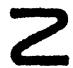
\includegraphics[keepaspectratio]{images/part002_a77d6c20.jpg}}

另一方面，当 A 是闭集时，即使 B 也是闭集，AB 也未必是闭集（参看 § 4 第 1 目命题 1 的推论 1）。

* 例如，在实直线 \(\mathbf{R}\) 的加法群中，有理整数组成的子群 \(\mathbf{Z}\) 是闭的，子群 \(\theta\mathbf{Z}\)（由全体整数倍 \(n\theta\)（\(\theta\) 为一无理数）组成）也是闭的；但子群 \(\mathbf{Z} + \theta\mathbf{Z}\)（\(\mathbf{R}\) 的），即实数 \(m + n\theta\)（其中 \(m\) 与 \(n\) 取遍一切整数值）组成的集，在 \(\mathbf{R}\) 中不是闭的，这一点我们将在第五章 § 1 中看到。

又，设 A 是 \(\mathbf{R} \times \mathbf{R}\) 的加法群中由全体点对 \((x, y)\)（满足 \(x \geqslant 0\) 与 \(0 \leqslant y \leqslant 1 - \frac{1}{x + 1}\) 的）组成的子集；并设 B 是当 x 取遍 R 时全体点对 \((x,0)\) 组成的集。A 与 B 都是闭的，但 \(A + B\) 是由全体点对 \((x,y)\)（满足 \(0 \leqslant y < 1\) 的）组成的集，它在 \(R \times R\) 中不是闭的。

设 X 是拓扑空间，f 与 g 是 X 到拓扑群 G 中的两个映射。若 f 与 g 在 X 的一点 \(x_{0}\) 处连续，则由第一章 § 2 第 1 目定理 2，\(\overline{f}^{1}\) 与 \(fg\) (*) 也连续。特别地，X 到 G 中的连续映射组成 X 到 G 的一切映射所成的群 \(\mathbf{G}^{\mathbf{x}}\) 的一个子群。

又，设 \(f\) 与 \(g\) 是集合 \(\mathbf{X}\)（由滤子 \(\mathfrak{F}\) 装备的）到 Hausdorff 拓扑群 \(\mathbf{G}\) 中的两个映射。若 \(\lim_{\mathfrak{F}} f\) 与 \(\lim_{\mathfrak{F}} g\) 存在，则 \(\lim_{\mathfrak{F}} \overline{f}^1\) 与 \(\lim_{\mathfrak{F}} fg\) 也存在，并且我们有（第一章 § 7 第 4 目命题 9 的推论 1）

\[
\lim _ {\mathfrak {F}} \overline {{f}} ^ {- 1} = (\lim _ {\mathfrak {F}} f) ^ {- 1},\tag{1}
\]

\[
\lim _ {\mathfrak {F}} f g = (\lim _ {\mathfrak {F}} f) (\lim _ {\mathfrak {F}} g).\tag{2}
\]

当 G 是写成加法形式的交换群时，公理 (GT') 表明 \((x, y) \to x - y\) 是连续映射。若 f 与 g 是拓扑空间 X 到 G 中的映射，并且在一点 \(x_{0}\) 处连续，则 f - g 在该点连续。公式 (1) 与 (2) 可以类似地改写。
